\documentclass[unicode,master,pdfcover]{fzuthesis} %pdfcover为可选项,博士doctor,硕士master
\usepackage{fontspec,color,array,longtable,graphicx} 
\usepackage{anyfontsize} %消除字体警告
\usepackage{enumitem}
\usepackage{tabularx}
\newcolumntype{M}[1]{>{\centering\arraybackslash}p{#1}}
\newcolumntype{L}[1]{>{\left\arraybackslash}m{#1}}
%%%%%%%%%%%%%%%%%%%%%%%%%%%%%%%%%%%%%%%%%%%%%%%%%%%%%%%%%%%%%%%%%%%%%%%%%%%%%%%%%%——by MCH

%参考文献设置
\usepackage[backend=biber,style=gb7714-2015,gbalign=gb7714-2015,gbpub=false,gbnamefmt = lowercase]{biblatex}
\addbibresource[location=local]{mybibfile2.bib} % bib文件,由参考文献的BibTeX组成
%页眉页脚设置
\usepackage{fancyhdr}
\usepackage{listings}
\usepackage{xunicode}
\renewcommand{\lstlistingname}{列表}
\pagestyle{fancy}
\fancyfoot[C]{\headfont\thepage}
\renewcommand{\chaptermark}[1]{\markboth{\chaptername\ #1}{}}
\renewcommand{\sectionmark}[1]{\markright{\thesection\ #1}}
\fancyhead[RE]{}
\fancyhead[RO]{}
\fancyhead[LE]{}
\fancyhead[LO]{}
\fancyhead[CO]{\headfont{非视距可见光成像定位技术研究}}%页眉标题奇页
\fancyhead[CE]{\headfont{福州大学工程硕士学位论文}}% 页眉标题偶页
\renewcommand{\headrulewidth}{1pt}%页眉线条粗细
\renewcommand{\footrulewidth}{0pt}%页脚线条粗细
%%%%%%%%%%%%%%%%%%%%%%%%%%%%%%%%%%%%%%%%%%%%%%%%%%%%%%%%%%%%%%%%%%%%%%%%%%%%%%%%%%
\usepackage[unicode=true,bookmarks=true,bookmarksnumbered=true,bookmarksopen=false,breaklinks=false,pdfborder={0 0 1},backref=false,colorlinks=true]{hyperref}
\hypersetup{
	linkcolor=black, anchorcolor=black, citecolor=black, filecolor=black, menucolor=black, urlcolor=black, pdfstartview=FitH}% 黑白,提交版

\makeatletter
%%%%%%%%%%%%%%%%%%%%%%%%%%%%%% LyX specific LaTeX commands.
\providecommand{\LyX}{\texorpdfstring%
	{L\kern-.1667em\lower.25em\hbox{Y}\kern-.125emX\@}
	{LyX}}
%% Because html converters don't know tabularnewline
\providecommand{\tabularnewline}{\\}
\makeatother
\begin{document}
	
	\maketitle	
	\frontmatter	%此后为罗马数字页码,页面类型为plain
	
\begin{abstractCN}

随着物联网 (IoT) 的快速发展,基于位置的服务变得越来越重要,尤其是在室内环境中,全球卫星导航系统 (GNSS) 信号受到墙壁的遮挡衰减严重,无法满足室内定位的需求。可见光定位 (VLP) 由于其精度高、成本低等优点,在多种室内定位技术中备受关注。特别是以图像传感器 (IS) 为接收端的可见光成像定位 (IS-VLP) 系统,由于 IS 的快速普及,有很大的市场潜力。然而,传统的 VLP 依赖于直接视距 (LOS) 路径,并且需要在有限的视场角内同时捕捉大量的发光二极管(LED) ,使其无法应对各种复杂多变的室内场景。 为了解决这两个主要的挑战,同时考虑到图像传感器的抗干扰性能更好,本文提出了一种仅需一个LED利用一次反射光进行定位的非视距可见光成像定位(NLOS IS-VLP)系统。

本文所提出的NLOS IS-VLP 系统可分为两个模块,包括一个用于接收 LED 位置信息的非视距光学相机通信 (NLOS OCC) 系统和一个可见光成像定位 (IS-VLP) 系统。其中,NLOS OCC 系统是一种以IS为接收端基于NLOS链路的可见光通信(VLC)系统。IS-VLP 系统主要利用计算机视觉(CV)算法实现定位,在本文中主要是利用重投影误差最小化算法来实现位置估计的。


本文给出了两种不同的NLOS IS-VLP系统实现方案。第一种方案提出了一种亮度分布模型,它可以用来表示一次反射光在图像传感器上的亮度分布情况,利用这种亮度分布模型,可以证明在仅有一个LED时,图像传感器上捕捉到的两个高光点可以被视为是两个虚拟的LED通过LOS在图像传感器上面的投影。其中,这两个虚拟LED的位置被证明是LED在反射面的投影和关于反射面的对称点。在得到LED的坐标和高光点的像素坐标之后,可以构建基于两个虚拟LED的LOS IS-VLP系统。第二种方案使用双目相机捕捉LED关于地面对称点,由于双目立体视觉算法可以实现在已知一个点在左右目图像上的像素坐标的情况下,计算其在相机坐标系的坐标,在惯性测量单元(IMU)的辅助下又可以获得相机的姿态。由此,很容易实现基于单灯的NLOS IS-VLP系统。

本文通过实验,测试和分析了这两种方案的性能。并且总结了所提出的NLOS IS-VLP系统的待改进之处,同时也给出了后续改进的方法。最后,对VLP系统的发展进行了展望。
 
\end{abstractCN}
	

\keywordsCN{室内定位;可见光通信;可见光定位;视距;非视距}


\begin{abstractEN}

With the rapid development of the Internet of Things (IoT), location-based services become more and more important, especially in indoor environments, where the Global Navigation Satellite System (GNSS) signals are severely attenuated by walls and cannot meet the needs of indoor positioning. Visible Light Positioning (VLP) has attracted much attention among various indoor positioning technologies due to its high accuracy and low cost, especially, the Image sensor (IS) based Visible Light positioning (IS-VLP) system.  It has great market potential due to the rapid popularization of IS. However, traditional VLP relies on  line-of-sight (LOS) path and requires capturing a large number of light-emitting diodes (LEDs) within a limited field of view, making it unable to cope with various complex and variable indoor scenarios. To address these two major challenges, considering the better interference resistance of IS, this paper proposes a non-line-of-sight (NLOS) IS-VLP  system that only requires a single LED to use the first reflected lights for positioning.

The NLOS IS-VLP system proposed in this paper can be divided into two modules, including a NLOS optical camera communication (OCC) system for receiving LED position information and a IS-VLP system. The NLOS OCC system is a visible light communication (VLC) system based on NLOS links with IS as the receiver. The IS-VLP system mainly uses computer vision (CV) algorithms to achieve positioning, which in this paper is mainly using the reprojection errors minimization algorithm to achieve position estimation.

This paper presents two different schemes for implementing the NLOS IS-VLP system. The first scheme proposes a luminance distribution model (LDM), which can be used to describe the luminance distribution of the first reflected lights on the IS. Using this LDM, it can be proved that when there is only one LED, the two highlights captured on the IS can be regarded as the projections of two virtual LEDs on the IS through LOS. The positions of these two virtual LEDs are proved to be the projection of the LED on the reflective surface and its symmetrical point about the reflective surface. After obtaining the coordinates of the LED and the pixel coordinates of the two highlights, a LOS IS-VLP system based on the two virtual LEDs can be constructed. The second scheme uses a stereo camera to capture the symmetrical point of the LED about the ground. Since the stereo vision algorithm can calculate its coordinates in the camera coordinate system when the pixel coordinates of the symmetrical point  in the left and right images are known, and the camera pose can be obtained with the help of an inertial measurement unit (IMU). Thus, it is easy to implement the NLOS IS-VLP system based on a single LED.

This paper tests and analyzes the performance of these two schemes through experiments. And summarizes the areas for improvement of the proposed NLOS IS-VLP system, and also gives the methods for subsequent improvement. Finally, it looks forward to the development of VLP system.



\end{abstractEN}

	

\keywordsEN{\textbf{Indoor positioning; Visible light communication (VLC); Visible light positioning (VLP); Line-of-sight (LOS); Non-line-of-sight (NLOS)}}
 % 中英文摘要
	%%%%%%%%%%%%%%%%%%%%%%%%%%%%%%%%%%%%%%%%%%%%%%%%
	% 目录、表格目录、插图目录这几个字本身的大纲级别是一级的,即和章名有相同的字号字体。目录表的内容通过titletoc宏包在。cls文件设置了。
	%\cleardoublepage % pdfbookmark可能需要这一条才能正常工作
	\pdfbookmark{\contentsname}{toc} %为目录添加pdf文件书签
	\tableofcontents	%目录
	%\listoffigures	%插图目录(可选)
	%\listoftables	%表格目录(可选)
	
	%%%%%%%%%%%%%%%%%%%%%%%%%%%%%%%%%%%%%%%%%%%%%%%%%
	%\include{symbols}	% 符号对照表(可选)
	%\include{abbreviation} 	% 缩略词(可选)	
	
	\mainmatter %此后为阿拉伯数字页码
	
    %%%%%%%%%%%%%%%%%%%%%%%%%%%%%%%%%%%%%%%%%%%%%%页眉页脚设置 ——by MCH 
    \fancypagestyle{plain}{
    	\pagestyle{fancy}
    }	% 每章的第一页会默认使用plain,没有页眉。通过重定义plain为fancy解决
    \pagestyle{fancy}	%设置页眉页脚为fancy
    %%%%%%%%%%%%%%%%%%%%%%%%%%%%%%%%%%%%%%%%%%%%%%分章节,结合导言区的\includeonly命令可仅编译部分章节,编译时不用切换界面,直接在相应章节编译即可。
	\chapter{绪论}

\section{研究背景与意义}
基于位置的服务(Location Based Serve, LBS)不管是在工业还是民用领域都扮演着非常重要的角色,例如物流管理、航道规划、智慧交通、自动驾驶以及智能家居等\cite{iot-lbs}。在室外环境中,全球导航卫星系统(Global Navigation Satellite System, GNSS)诸如美国的GPS (Global Positioning System)以及中国的北斗卫星导航系统等都能够提供高精度低成本的定位服务,基本上满足了各种室外活动的需求。然而,在复杂多变的室内环境中,GNSS信号衰减严重导致定位精度下降,以至于很难满足室内定位的需求\cite{裴凌2017室内定位技术与应用综述,ips-gnss-mehrabian2023sensor}。近年来,物联网的飞速发展,一方面,室内环境如家庭、工厂以及商超等对位置服务有需求的终端设备数量指数级增长;另一方面,室内环境下对定位精度以及稳定性的要求也非常高。针对室内环境对位置服务在数量和质量上的需求,如何在复杂多变的室内环境下提供高精度、低成本以及稳定的位置服务是一个重要的挑战。

为了克服上述挑战,一些室内定位系统(Indoor Positioning System, IPS)被设计出来,它们利用各种不同的无线信源来发射信标,其中主要分为以下四类:射频信源、音频信源、磁源以及光源\cite{陈锐志2017基于智能手机的室内定位技术的发展现状和挑战,ips-wahab2022indoor}。

目前,使用射频信号的IPS种类最多,它们基本上都是工作在不同频段以及拥有不同的编码方案,如常见的蓝牙、WiFi (Wireless Fidelity)以及ZigBee、超带宽、蜂窝网络、伪卫星等\cite{闫大禹2019国内室内定位技术发展现状综述}。

其中,伪卫星通过地面基站发射类似GNSS信号来定位,优点是覆盖范围广,精度高,但是系统复杂和成本高昂\cite{李占营2018基于伪卫星技术的室内定位系统硬件设计及实现}。

蓝牙、ZigBee、WiFi、以及超带宽 (Ultra-wide-band, UWB) 四种方案,都是基于短距离无线通信技术,需要部署多个节点来覆盖室内所有区域,一般定位的精度跟信标节点的布局方式以及密度有关。其中,基于WiFi的IPS主要是通过指纹法和测距法来实现定位\cite{wifi}。测距法通过将不同信标节点的接收信号强度(Received Signal Strength, RSS)转化为距离来估计接收端的位置,这种方法相对于指纹法不需要建立和维护指纹数据库并且拥有更高的精度,但是由于室内环境的复杂多变,因此很难进行准确的信道建模,从而无法准确的构建信号强度与距离之间的关系。随着IEEE802.11标准的更新,增加了通过计算接收端与信标节点之间的报文时间戳来估算信标节点到接收端的时间,从而估计两者之间的距离,这种方法不需要对信道进行建模,但是对时间同步有很高的要求。基于蓝牙的IPS和基于WiFi的IPS类似,都可以通过指纹法和测距法来实现定位\cite{bluetooth}。此外,在蓝牙5.1协议中增加了方向测量的方案,补充了通过多天线阵列的信号相差来测量离开角度和到达角度的功能,因此基于蓝牙5.1的IPS系统可以使用到达角度 (Angle of Arrival, AOA)来定位。基于蓝牙的IPS拥有低功耗、低成本的优点,但是通信距离短导致需要更密集的信标节点。为了增加通信距离需要提高广播信道的功率。基于ZigBee的IPS主要是通过指纹法来进行定位,拥有低成本、低功耗等优点。然而,由于IEEE 802.15.4标准低速率、大延迟的缺点,基于ZigBee的IPS更容易受到噪声的干扰以及多径效应的影响导致定位精度下降,并且很难满足实时定位的要求\cite{ZigBee}。UWB由于其高带宽的特点拥有非常高的传输速率,又因为发送的是窄脉冲的数据包,因此拥有很高的时间分辨率\cite{uwb}。因此,基于UWB信号的IPS通过使用TOA (Time of Arrival, TOA)的定位方法可以获得非常高的精度。然而,由于极高的时间分辨率,将导致在非视距下的信号延迟可能使系统无法正常工作。除此之外,也可以通过部署多个UWB节点来测量到达角度,从而使用AOA定位方法。UWB定位拥有非常高的精度以及速度,但是成本也非常高。

基于蜂窝网络的IPS通过主要是通过邻近匹配法来判断接收端到附近基站的位置\cite{LTE}。作为最新的蜂窝移动通信技术,5G(毫米波)技术的大带宽和大规模天线阵列带来了更高的通信速率和更低的延迟,一方面可以提高基于TOA技术的定位精度,另外一面,大规模天线阵列可以提高角度测量的精度从而提高基于AOA定位方法的精度。除此之外,高频信号和低延迟更有助于抵抗多径效应。然而,基于蜂窝网络的IPS主要的挑战是定位精度、成本与基站密度的问题。基于5G技术的IPS拥有很高的定位性能与5G基站的密集程度有关,但是更高的功耗以及建造成本也不容忽视\cite{5g}。

使用音频信号的IPS根据音频的波段分为超声波定位和音频定位,都是通过计算时间来估计距离,前者是计算超声波经过反射回到出发点的时间\cite{室内超声波定位系统},后者计算的是声音从基站到达接收端的时间\cite{曹帅2020面向智能移动终端的音频室内定位关键技术研究}。由于声音的传播速度相较于电磁波非常慢,因此对时间同步的精度要求不高,但是受多径效应和非视距的影响非常严重。并且,由于超声波频率容易受到温度影响,因此对待定位设备所处的环境以及其数量有要求,总体来说,系统复杂成本较高。音频定位由于工作频率在人耳可听的范围内,环境声音可能会对其造成干扰。

利用磁源进行室内定位的有两种主流方案,第一种是利用地球磁场进行定位,另外一种是认为铺设磁源设备进行定位。前者根据地球磁场在地理位置上的差异性来构建指纹数据库,接收端可以根据采集到的磁场强度的方向来匹配指纹库从而判断自己的位置。但是由于室内环境中小范围的磁场差异不明显导致定位误差较大。因此,在很多物流场地,通过人为在地面铺设磁源设备来增加区域的磁场差异性,从而提高定位精度。同样的,定位精度取决于磁源设备的密集程度\cite{周家鹏2019地磁室内定位技术研究,ips-wang2023improved}。

根据光的波长可以将基于光源信号的IPS分为红外线定位和可见光定位(Visible Light Positioning, VLP)。红外线定位首先待定位物体通过周期性的发送的包含特殊标记的红外信号给探测器,探测器在探测到红外信号后将自己的信息发给服务器,服务器从而知道带定位物体的位置,这种定位方法其实也是邻近匹配法,定位精度不高,目前很少使用。

VLP作为一种最新的室内定位方法,通过可见光通信(Visible Light Communication, VLC)技术来实现对信标的接收\cite{vlp-abdalmajeed2023improved,vlp-sen20233d}。首先,发送端通过对位置坐标进行编码然后按照一定的调制方案来驱动发光二极管(Light Emitting Diode, LED)发送调制光信号,接收端通过光电探测器 (Photo-diode, PD) 或者图像传感器(Image Sensor, IS)捕捉随时间变化的光强度信号\cite{ips-pd-is-liu2022efficient}。通过解调解码来获取发送端的坐标,与此同时,通过接收到的信号强度估计接收端和发送端之间的几何关系,从而估计自身的位置。VLP凭借下述的优越性,在IPS中非常具有潜力:
\begin{enumerate}[topsep = 0 pt, itemsep= 0 pt, parsep=0pt, partopsep=0pt, leftmargin=20pt, itemindent=0pt, labelsep=6pt, label={(\arabic*)}] 

    \item 可见光的频谱非常宽,因此VLC拥有无限制的频谱资源。这对于基于射频信号以及音频信号的IPS来说,非常的关键。考虑到物联网的快速增长,频谱资源日益紧张,当海量终端同时运行时,可能存在竞争频谱资源导致的通信阻塞、链路中断等问题。
    \item 部署更多信源节点的成本很低。由于LED工艺的发展,LED造价低、功耗低、寿命长,安装简单,相对于其他IPS来说,将不再考虑由于部署更多节点带来的成本问题,因而VLP系统的成本可以控制在非常低的一个水平。
    \item VLP在物理层有更高的安全级别。由于可见光直接视距(Line-of-sight, LOS)传播特性,将保证物理层信号不容易被监听。
    \item VLP系统的定位精度非常高。在目前已经实现的很多VLP系统中,可以实现低成本的同时具有很高的定位精度。
\end{enumerate}

表\ref{tab:positioning-systems} 总结了目前主要的一些IPS的定位方法以及优缺点。考虑到VLP在频谱资源、成本以及定位精度等方面与基于射频信源、音频信源以及磁源的IPS有很大的优越性,我们认为室内VLP系统在复杂多变的室内环境下提供高精度、低成本以及稳定的位置服务最有潜力。
\begin{table*}[!htbp]
  \centering 
  \small
  \caption{不同类型的室内定位系统对比}  
  \label{tab:positioning-systems}  
  \begin{tabularx}{\textwidth}{lccc}
    \toprule
   \textbf{信源类型}   &   \textbf{定位方法}     & \textbf{优点}     &\textbf{缺点} \\
    \midrule
    伪卫星    &   TOA   &   精度高,覆盖范围广    &     系统复杂,成本高昂  \\
    
    WiFi    &   RSS测距   &   功耗低,易部署  & 信道建模比较复杂,影响精度  \\
    WiFi    &   TOA   &   功耗低,易部署  & 时间同步要求高  \\

    蓝牙    &   AOA   &   成本低,功耗低,易部署  & 覆盖范围小,需要密集部署  \\
    
    ZigBee    &   指纹对比   &   成本低,功耗低   &  易受噪声和多径的影响,实时性低  \\
    
    超带宽    &   TOA   &   精度高    &成本高,受非视距影响严重  \\
    
   蜂窝网络    &   邻近匹配   &   简单,易实现    &精度低,受多径影响  \\
   
   5G毫米波    &   TOA、AOA   &   精度高,抗多径干扰    &成本高  \\

   音频    &   TOA、TDOA   &   成本低,易部署    &受多径和环境声影响  \\
   
   磁场 &   指纹匹配   &不受遮挡的影响       &建立和维护指纹库成本高  \\
   
   可见光 &   TDOA、CV   &精度高、成本低       &受非视距影响  \\
   
    \bottomrule
  \end{tabularx}%
\end{table*}%



\section{研究现状与挑战}
\subsection{可见光通信的研究现状}
VLC是一种通过对频率在400-800THz的可见光进行调制来传输数据的通信技术,凭借其安全、无电磁辐射、免频谱授权等优点,是最有潜力的下一代无线通信技术之一\cite{vlc-sejan2023comprehensive}。可见光波谱如图\ref{fig:spectrum}所示,远大于无线电频谱。
\begin{figure*}[!htbp]
  \centering
  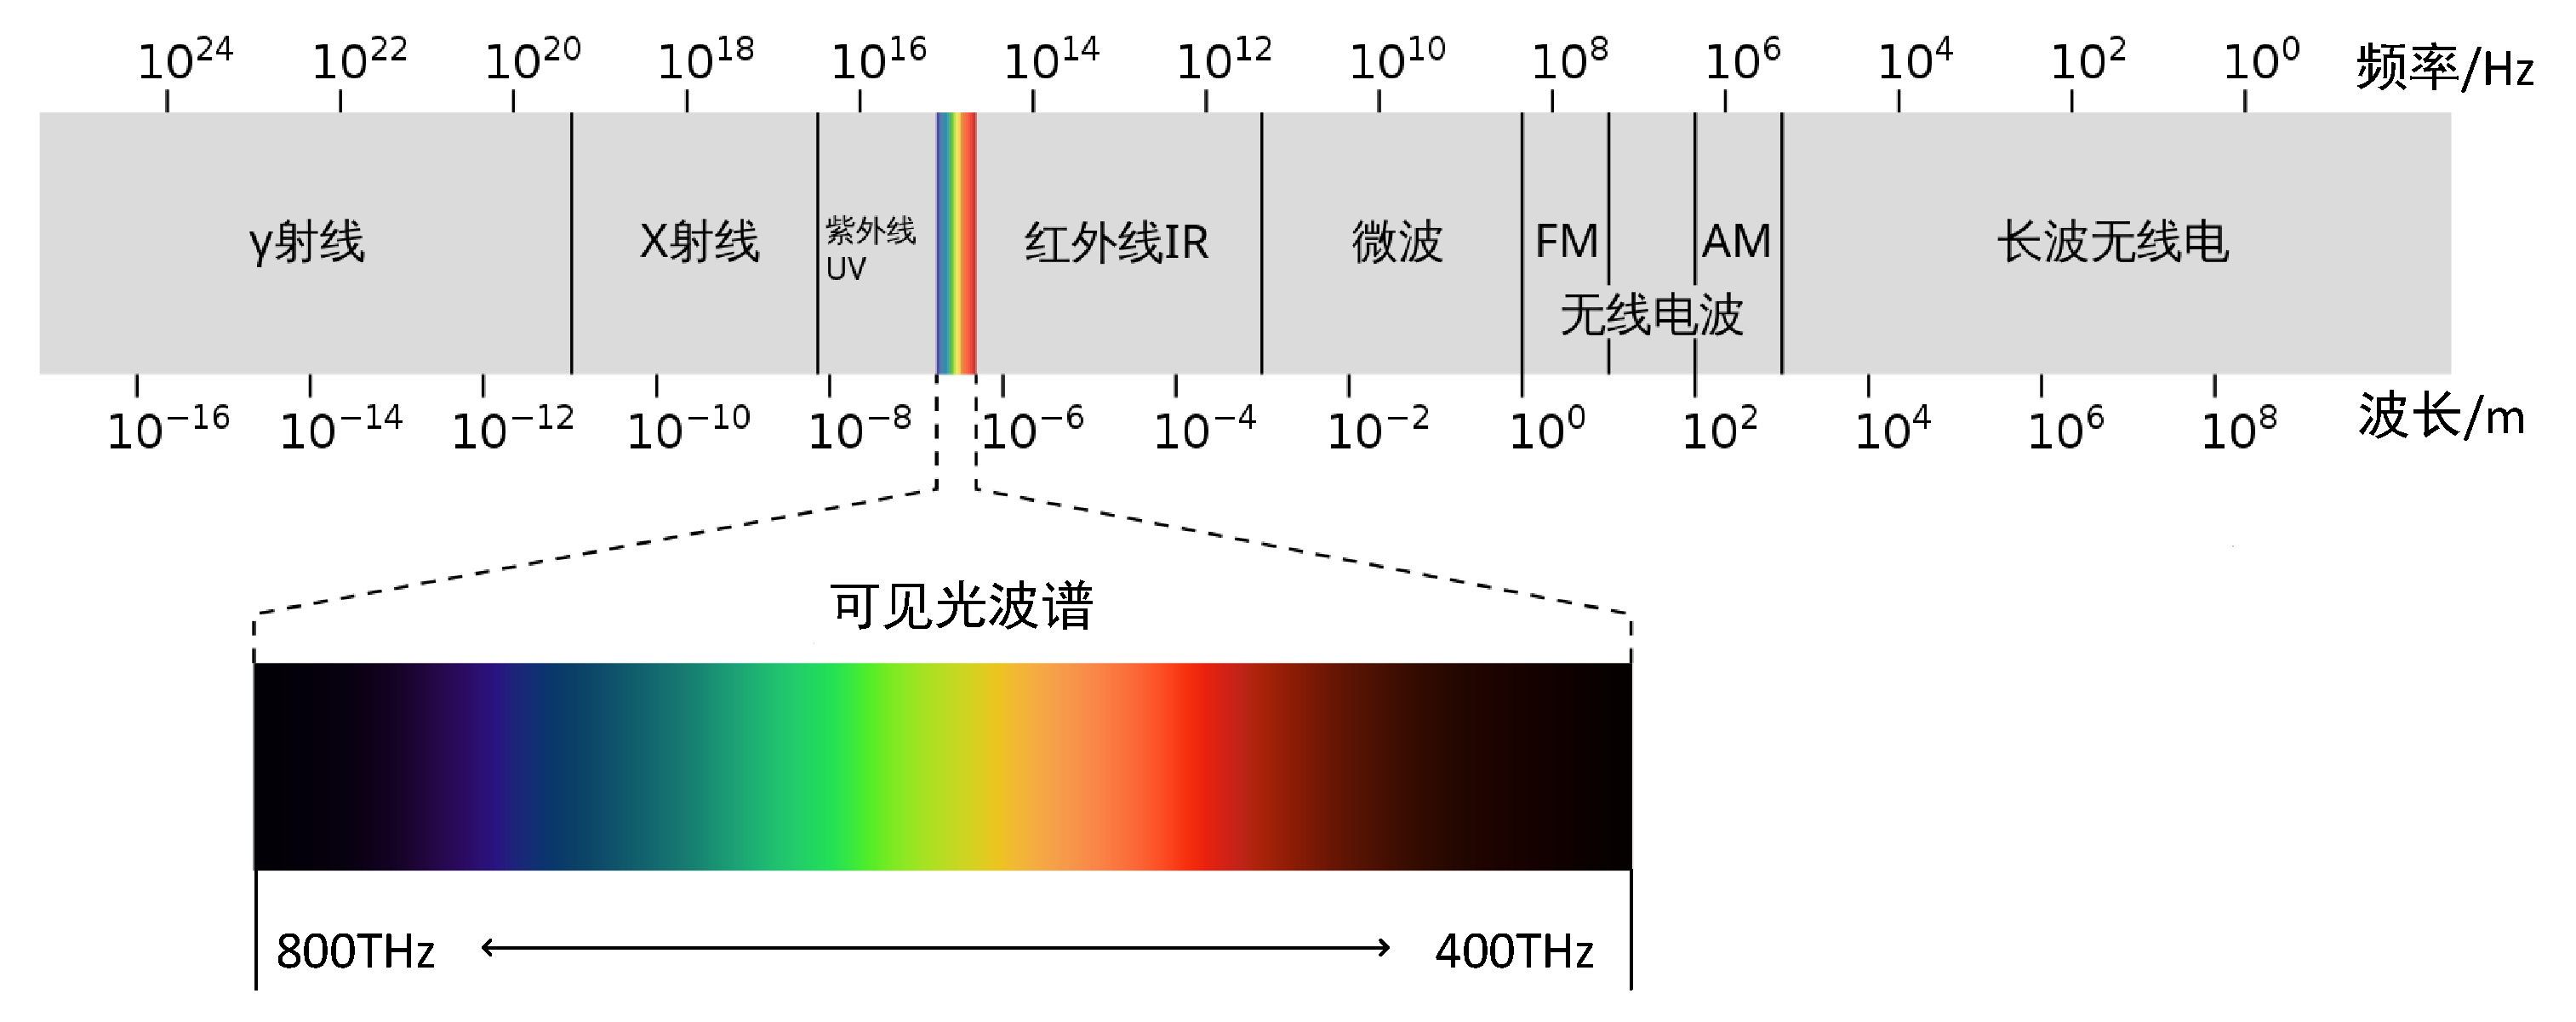
\includegraphics[width=\linewidth]{FIG/Eletornic spectrum.pdf}
  \caption{可见光波普}
  \label{fig:spectrum}
\end{figure*}


虽然古代军事上早就应用了VLC来传输信息,但是现代意义上的VLC概念最早是在1999年由香港大学G.Pang教授提出来的\cite{1211-vlc1999}, G.Pang教授在实验中利用VLC技术实现音频信号传输。

2000,日本中川实验室Tanaka等人提出使用白色LED的照明设备应用于无线家庭链路中的接入点,并通过仿真验证了该方案的可行性\cite{1212-vlc2000}。随即,日本研究人员开始意识到VLC的潜力以及存在的巨大应用前景,相应的,日本政府在2003年的时候成立了“可见光通信协会 ”,旨在助力VLC系统产业化。2004年,日本学者Komine等人讨论了干涉和反射对VLC系统的影响,对VLC信道研究奠定了理论基础\cite{1213-vlc2004}。

在之后的几年时间里,大量学者对VLC系统进行了研究,VLC系统的通信速率从几kbps快速发展到了几十Mbps,特别是2009年英国牛津大学的Minh等人考虑到了普通白光LED有限带宽对VLC速率的限制,通过蓝色滤波结合简单的接收机均衡,可以实现50MHz的带宽和100Mbps基于开关键控不归零调制的数据链路\cite{1214-vlc2009}。与此同时,欧洲政府开始启动1Gbps VLC系统研究项目,将VLC技术是为家庭无线接入技术的重要研究对象。由于VLC的快速发展,IEEE于2011年发布了关于VLC的IEEE 802.15.7协议,该协议作为第一个VLC国际标准,定义了用于VLC的PHY层和介质访问控制层,并承诺了足以支持音频和视频多媒体服务的数据速率。同年,英国爱丁堡大学数字通信研究中心的Harald Hass 教授提出了LiFi (Light-fidelity) 的概念,认为VLC可以做到低功耗的同时实现1Gbps以上的高速通信\cite{1215-vlc2011}。

然而,硬件的性能以及传统的调制方式限制了高速VLC的发展。为了提高VLC的速率,一方面,大量的工作开始研究发射端、接收端的硬件性能,包括发射端器件如RGB-LED、磷光LED、硅基LED(Si-LED)、micro-LEDs阵列以及微型激光二极管(Laser Detector, LD)等等\cite{1216-vlc-rgb,1217-vlc-blue-led,1218-vlc-si-led,1219-vlc-microled,12110-vlc-ld},和接收端光电探测器如PIN阵列、微型探测器阵列(Micro-photo-detector, μPD)、雪崩式光电二极管(Avalanche Photo-diode, APD)、单光子雪崩二极管(Single-photon Avalanche Diode, SPAD)等\cite{12111-vlc-pin,12115-vls-upds,12112-vlc-apd,12114-vlc-spad,12113-vlc-spad}。另外一方面,针对VLC先进调制技术的研究也非常多,包括波分复用(Wave Division Multiplexing, WDM),正交频分复用(Orthogonal Frequency Division Multiplexing, OFDM),无载波幅度相位调制(Carrier-less Amplitude and Phase, CAP)和离散多音(Discrete Multi-tone, DMT)等\cite{12116-vlc-wdm,12117-vlc-ofdm,12118-vlc-ofdm,12119-vlc-cap,12120-vlc-cap,12121-vlc-cap,12122-vlc-dmt}。近十年,通过使用高性能的器件和先进的调制技术,国内外大量的VLC研究工作表示取得了几Gbps到几十Gbps的通信速率,例如英国爱丁堡大学数字通信研究所LiFi研发中心在2017年通过紫光微型LED阵列实现了11.95Gbps的数据传输速率\cite{12123-vlc-11.95G},该研究所在2019年通过WDM和OFDM结合,使用低成本的LED实现了15.73Gbps的通信速率\cite{12124-vlc-15.73G}。英国牛津大学工程科学学院在2018年提出了一个四色多路复用高速VLC系统,基于激光二极管的白光通信链路和宽视场角覆盖,实现了35Gbps的通信速率\cite{vlc-nature-35Gb}。我国科研院所在高速VLC系统的设计研发上也取得了很多重要成果,其中复旦大学迟楠教授团队在2015年通过WDM和CAP调制最早实现了VLC系统达到8Gbps以上速率\cite{vlc-chinan-8Gb},在2020年通过硅基多色LED阵列实现了20.09Gbps速率的领先水平\cite{vlc-chinan-20.09Gb},在2022年使用GaN超级发光二极管(Super Laser Detector, SLD),在国际上率先实现了在单芯片传输速率达到4.57Gbps的速率\cite{vlc-chinan-4.57Gb}。

IEEE 802.15.7协议规定VLC被作为一种短距离通信技术,大量的VLC实验演示系统通信距离都在几十厘米到几米的距离。虽然通过使用激光发射器作为发射端可以实现几十公里的通信距离,但是由于激光链路在远距离对准上的问题,只能应用在一些特定场合,并且由于覆盖范围较小,很难作为一种大规模商用的无线接入方案。目前在使用LED作为发射端的自由空间VLC系统中,复旦大学信息科学与技术学院电光源研究所设计了一种基于多色串联LED阵列的VLC系统,实验结果表明,在15.78Gbps的速率下实现了最远13m的远距离通信\cite{vlc-longdistance-13m}。值得注意的是,这是到目前为止基于LED的VLC系统所能达到的最远通信距离。

大量研究高速远距离VLC系统的工作为VLC的应用推广奠定了理论基础。与此同时,一些学者开始考虑将VLC技术应用于如智慧交通\cite{vlc-v2x-1,vlc-v2x-2}、室内VLP\cite{vlc-vlp-1,vlc-vlp-2}、水下可见光通信\cite{vlc-uwoc}等等场景。除此之外,考虑到相机在商业市场的普及程度,2012年英国爱丁堡大学的研究人员首次使用智能手机摄像头为接收端的VLC系统,实现了最大3.1Kbps的通信速率\cite{vlc-occ-first2012}。此后,这种为以相机为接收端的VLC被称为光学相机通信(Optical Camera Communication, OCC),开始受到了大量的关注\cite{vlc-occ,vlc-occ-2}。OCC系统通信速率与相机帧率正相关,目前已知的OCC系统可以做到的最高的通信速率是44.03kbps \cite{vlc-occ-5}。

虽然大量的研究工作在积极的推广VLC,但是VLC距离实用化还存在一定的距离,这主要是因为VLC面临几个主要的挑战,如LED的非线性、环境光干扰、上行链路以及视距等\cite{vlc-challenges}。其中,最主要的挑战是LOS受阻,在这种情况下,系统可能无法工作。目前,比较好的解决方法是通过反射光来进行通信,这种被称为非视距(Non-line-of-sight, NLOS) VLC。由于反射光信号的低信噪比,图像传感器在抗噪方面的特性由于PD,因此NLOS OCC受到更多的关注,特别是英国诺桑比亚大学Ghassemlooy教授团队在此方向上做了大量的工作\cite{vlc-nlos-1,vlc-nlos-2}。


\subsection{可见光定位的研究现状}
VLP是一种基于VLC的室内定位技术,通用的架构一般是通过调制驱动LED来发送包含位置信息的光信号,使用被固定在待测物体上的接收端来捕捉光信号,通过解调解码技术来获得LED的位置,然后使用位置估计算法来判断接收端的位置。

日本庆应义塾大学的M.Yoshino和C.Sertthin等人最早开始VLP的研究,2007年M.Yoshino等人基于VLC技术,通过使用IS和LED实现了定位\cite{is-first-1,is-first-2};2008年,C.Sertthin等人通过使用VLC技术来发送LED的位置信息,然后对接收端进行位置估算\cite{vlp-01-cs,vlp-02-cs},在只需要几个LED的情况下可以实现较高精度的室内定位。在此之后,VLP作为室内定位技术之一,受到了广泛的研究。

与VLC系统一样,按照接收端是PD还是IS,VLP系统也分为两类,分别是可见光成像定位(Image Sensor Based VLP, IS-VLP)和可见光非成像定位。一方面,PD的采样频率远高于IS,因此可以实现更高的时间分辨率。而且PD采集信号强度更精确,成本也比较便宜。另外一方面,IS可以看成是微型PD阵列,因此IS接收的是二维空间上的光强度信号,从而更容易测量AOA和LED的2D位置信息,并且搭载IS的终端设备数量在近十年来快速增加。因此,对基于这两种类型的接收端的可见光定位系统都有很大的应用前景。

VLP定位算法主要分为几何测量、指纹对比、接近度匹配以及计算机视觉(Computer Vision, CV)等几个类型,其中几何测量又可以分为距离测量和角度测量,前者包含RSS、TOA以及到达时间差(Time Difference of Arrival, TDOA)等,后者主要是测量AOA。除了计算机视觉算法是依赖于相机成像,其他类型的定位算法都可以和两种类型的接收端进行组合,从而实现多种类型的VLP方案\cite{vlp-class-cn}。已经有大量的研究成果表明,这些方案都可以实现较好的定位性能\cite{vlp-luo-2017-review}。

接近度匹配的思路跟蜂窝网络定位方法类似,都是根据接收端是否检测到来自某个LED的光信号来判断自己是否在此LED的覆盖范围内。当同时接收到多个LED的光信号的时候就代表接收端的位置在这些LED覆盖范围的重叠部分。这种接近度匹配的定位方法简单,但是定位精度比较低,在发射端数量比较多的时候需要考虑复用协议。目前,使用接近度匹配的方法的VLP系统取得的最好的性能是在5m$\times$5m$\times$3m的房间内使用9个LED和1一个PD达到了12.9cm 的 2D 定位精度\cite{proximity-12.9cm}。

指纹对比是一种基于空间差异性的定位方法,通过提前采集需要定位区域的位置相关数据例如光信号强度、颜色、频率等等构建数据库,接收端将采集到的信号与数据库进行比对,匹配程度越高代表自己所在的位置与指纹对应的区域越接近。这种方法前期构建数据库的工作量比较大,而且当发射端发生变化需要及时的更新数据库,人力成本较高,定位精度也依赖于指纹库的密集度。目前,基于PD的指纹对比VLP系统,最好的性能是使用4个LED阵列,在1m$\times$1m$\times$1.2m的房间里取得4.38cm 的2D定位精度\cite{fingerprinting-pd-1}。

根据VLC的信道模型,RSS可以跟接收端到发射端之间的距离建立关系从而判断自己跟发射端LED之间的关系,在接收到多个LED的信号强度之后,可以唯一确定接收端的位置\cite{vlp-pd-rss,vlp-9728724}。基于RSS的定位算法还有一种改进算法称为接收信号强度比(Received Signal Strength Ratio, RSSR),前提是需要接收端的接受平面与LED的发光平面平行,可以得到入射角与辐射角相同,从而抵消角度对距离与信号强度关系的影响。这种算法的优点是,可以直接将多个基站的接收功率比转化为距离比,进一步根据距离比确定位置,一方面简化了算法复杂度,另外一方面减小了辐射角造成的误差,提高了定位精度\cite{vlp-pd-rssr}。然而,一方面由于受到信号接收的准确性的影响,特别是容易受到环境光、反射光以及其他光源的干扰,另外一方面,由于室内环境复杂多样,导致信道建模比较复杂,目前大部分VLP演示系统的定位精度都在10cm左右。

基于TOA的定位算法原理比较简单,跟GPS定位类似,通过计算光信号从发射端到接收端的时间来计算两者之间的距离。就2D定位而言,当发射端的数量在三个以上并且同一高度时,就可以确定接收端的位置,此时接收端的位置可以看成是三个圆的交汇点,但是由于误差的存在,实际情况接收端的位置被约束在三个圆的一个重叠区域。对于3D定位来说,在同样考虑误差的情况下,接收端的位置被约束在三个球体的重叠空间里面,当发射端的数量增加时,所有球体的公共空间越来越小,3D得的精度也越来越高\cite{vlp-pd-toa}。TOA定位算法受到时间同步的影响,为了消除其带来的误差,一种基于TDOA的改进算法被应用到VLP。TDOA的原理是基于接收端到两个发射端的到达时间差可以转化成距离差。到两个发送端的距离差不变时,接收端的位置可以看成是在两条双曲线上。当有三对以上这样的发射器,接收端的位置就可以确定在这些双曲线相交的位置\cite{vlp-pd-tdoa}。就目前的一些研究成果来看,TOA、TDOA的定位精度依赖于发射端的数量,当发射端数量比较多时,3D的定位精度都可以做到几厘米。

根据接收到的可见光信号,可以计算接收端与发射端之间的相对夹角,从而确定接收端的位置,这种定位方法称为AOA。一般接收端都是使用PD阵列或者图像传感器来测量AOA。当使用PD阵列时,根据朗伯辐射模型,忽略PD尺寸和辐射角的影响,不同的PD接收到的信号强度与入射角度相关,因此通过估计位置对应的所有PD的RSS和实际的RSS的差值均方根最小化,可以估计接收端的位置\cite{vlp-pd-aoa}。在使用图像传感器为接收端时,根据针孔相机模型,在角度传感器辅助的情况下,很容易测量LED相对于相机的入射角度,从而判断出相机自身的位置\cite{vlp-is-aoa}。AOA定位算法不需要发射端之间的同步,并且由于光沿直线传播的特性,测量信号角度更方便。AOA定位算法整体来说相对复杂,但是定位精度较高。
\begin{figure*}[!t]
  \centering
  \includegraphics[width=0.8\linewidth]{FIG/VLP methods.pdf}
  \caption{可见光定位及优化方法}
  \label{fig:vlp-methods}
\end{figure*}

除了使用上述了这些定位方法,越来越多的研究工作开始考虑通过多种算法协作定位、多源融合以及多传感器融合定位\cite{zhuang2018survey}。对于协作定位来说,一方面可以通过两种定位算法的结果进行耦合来提高定位的精度,另外一方面,有时候单纯的依赖某一种算法无法实现3D定位,通过两种定位算法协作可以实现\cite{vlp-rss-aoa}。多传感器融合定位,最常见的是惯性测量单元(Inertial Measurement Unit, IMU)和IS组合,实现任意姿态下的3D定位,还有一些使用PD和IS融合的VLP系统。这种多传感器融合,利用各种传感器提供的信息进行互助,一方面可以提高定位的精度,另外一方面可以提高定位系统的鲁棒性\cite{vlp-fusionvlp,vlp-fusion-yang2022cga}。

在使用定位算法粗略估计出接收端的位置之后,由于定位结果一般存在较大的波动,因此一些研究工作通过使用滤波器技术对定位的结果进一步优化,常见的优化算法有卡尔曼滤波算法\cite{vlp-kf}、粒子滤波算法\cite{vlp-pf}。卡尔曼滤波器是一种线性滤波器,根据观测数据对系统状态进行最优估计,广泛的应用于定位系统中。粒子滤波算法通过随机样本来描述整体分布,通过随机样本对概率密度函数进行近似,可以用样本均值来代替积分运算来获取系统的最小方差,降低算法复杂度。粒子滤波器适用于非线性系统,广泛的运用于状态跟踪,在实时定位系统中作用较大。

近年来,随着机器学习的热潮,一些工作开始研究基于深度学习算法的VLP系统\cite{vlp-ml-tran2022machine}。特别是针对指纹对比的定位算法,机器学习可以提高指纹比对的准确性从而提高定位精度,同时,基于机器学习的VLP系统可以极大的提高系统的鲁棒性。需要注意的是,这些基于机器学习定位算法主要分为两类,一类是基于机器学习对定位结果进行优化,如循环神经网络,可以看成是一种优化算法\cite{vlp-ml-1,vlp-ml-RNN},另外一类是将LED的坐标与接收端坐标作为输入输出来训练模型,在通过VLC技术获取LED的坐标输入到模型之后,可以实现对定位结果的直接输出,比如强化学习和BP神经网络\cite{vlp-ml-2,vlp-ml-3,vlp-ml-RL}。图\ref{fig:vlp-methods}给出了VLP系统常见的定位以及优化方法。


\subsection{可见光定位系统面临的挑战}
VLP技术发展迅速,包括硬件系统、软件算法等方面有很大的提高,大量的演示系统都展示了在低成本的同时具有相对较高的定位精度。然而,VLP作为最具潜力的IPS,目前除了一些商业上的试点应用外,大部分关于VLP的演示系统依然停留在实验室研究阶段。本文将按照接收端的不同,分开讨论其主要原因。

对于基于PD的VLP系统来说:
\begin{enumerate}[topsep = 0 pt, itemsep= 0 pt, parsep=0pt, partopsep=0pt, leftmargin=20pt, itemindent=0pt, labelsep=6pt, label={(\arabic*)}] 

    \item 环境光源以及反射光的存在,对VLC系统的信号解调造成困难,特别是在低信噪比场景下。
    \item 整体来说基于PD的定位算法较为复杂抑或是成本较高。TOA对时间同步要求很高;AOA需要多个PD组成阵列,并且算法较为复杂;指纹对比需要大量的人力成本;接近度匹配定位精度不高;RSS对复杂环境的信道建模要求严格。相对来说,TDOA算法最适合基于PD的VLP系统,但是需要捕获足够数量的LED。
    \item 普通的LED带宽有限,大量的LED对系统的复用技术有很高的要求。
\end{enumerate}

对于IS-VLP系统来说:
\begin{enumerate}[topsep = 0 pt, itemsep= 0 pt, parsep=0pt, partopsep=0pt, leftmargin=20pt, itemindent=0pt, labelsep=6pt, label={(\arabic*)}] 

    \item 系统需要相机在短曝光模式下进行通信,长曝光模式定位,实际的过程中相机需要在两种模式之间快速切换较为困难,并且功耗较高。
    \item 系统的实现同样需要捕获足够数量的LED。当相机距离发射端太近时,有限的视场角内无法捕获足够数量的LED,而距离太远使得LED在图像上的光斑太小,无法显示足够的条纹数量用于解调LED的位置信息。
    \item 普遍来说,相机的帧率太低,实时定位难以实现。
\end{enumerate}

 除此之外,两种类型的VLP系统都必须面临的一个共同的挑战是阴影和阻挡。在这种情况下,光信号被阻挡,无法通过VLC技术获取LED的坐标从而导致定位系统无法正常运行。
 
 综上所述,一方面,如何在LOS受阻的情况下依然能够保证系统的正常运行,另外一方面,如何在只有少量的LED的情况下实现高精度3D定位,是VLP系统面临的两个最主要的挑战。



\section{本文主要研究内容和结构}
\subsection{研究内容}
首先,考虑到IS的以下优点,本文主要研究了IS-VLP系统:
\begin{enumerate}[topsep = 0 pt, itemsep= 0 pt, parsep=0pt, partopsep=0pt, leftmargin=20pt, itemindent=0pt, labelsep=6pt, label={(\arabic*)}] 

    \item 随着物联网的快速发展,使用COMS(Complementary Metal Oxide Semiconductor)相机的终端设备数量快速增加,这将为VLP的推广提供硬件基础。
    \item IS可以看成是micro-PD阵列,方便测量信号的到达角度,对于基于AOA算法的定位系统来说无需其他的方法来测量角度。
    \item IS在低信噪比场景下的抗干扰能力更好。
\end{enumerate}
在前面提及的NLOS OCC系统的基础上,本文提出了利用反射光进行IS-VLP,本文中称之为非视距可见光成像定位(NLOS IS-VLP)。本文主要的研究内容就是通过NLOS IS-VLP解决上述提及的室内VLP系统面临的两个主要的挑战。

本文将NLOS IS-VLP系统结构分为两个模块,包括一个NLOS OCC子系统和一个位置估计子系统。一方面,本文设计了一套NLOS OCC子系统,通过捕捉反射光信号来获取LED坐标;另外一方面,本文研究了如何在只有一个LED的情况下进行VLP的单点定位算法。通过将NLOS OCC和单点定位算法进行结合,本文提出的方案不仅克服了LOS链路被阻挡,并且在只有一个LED的情况下实现了3D NLOS IS-VLP。

最后,本文给出了两种基于单个LED的NLOS IS-VLP方案。

\begin{enumerate}[topsep = 0 pt, itemsep= 0 pt, parsep=0pt, partopsep=0pt, leftmargin=20pt, itemindent=0pt, labelsep=6pt, label={(\arabic*)}] 

    \item 通过实验观察,当只有一个LED打开时,图像传感器上会出现两个高光点。本文提出了一个基于双向反射率分布函数(Bi-directional Reflectance Distribution Function, BRDF)的亮度分布模型(Luminance Distribution Model, LDM)来描述这一现象。通过LDM,我们证明图像传感器上的两个高光点可以看成是两个虚拟LED通过LOS链路形成的投影,并且构建了两个虚拟LED与真实LED之间的位置关系。基于这两个虚拟的LED,我们实现了基于单灯的3D NLOS IS-VLP。
    \item 本文提出了一个使用单个LED和双目相机的室内3D NLOS IS-VLP系统。通过双目视觉原理,可以计算LED在相机坐标系中的坐标,在IMU的辅助下可以获取相机自身的姿态角,最后通过求解重投影误差最小化函数的最优解来估计位置。
\end{enumerate}



\subsection{文章结构}
本文基于模块化思路将全文分为六章,对室内VLP系统的研究背景以及发展现状进行了全面的回顾,对NLOS IS-VLP基本原理和实现方法进行了详细的阐述和总结,最后对室内VLP系统的未来的发展方向进行了展望。

第一章是绪论部分,将从研究背景、研究现状、研究挑战等角度对室内VLP系统进行全面的介绍,以及在此基础上给出了本文的研究内容的概括和文章结构。第二章分别给出NLOS IS-VLP系统的理论基础,根据NLOS IS-VLP系统架构将系统划分为两个模块,包括NLOS OCC系统的基础理论和NLOS IS-VLP算法原理。第三章给出了NLOS OCC系统设计,NLOS OCC系统作为作为NLOS IS-VLP系统的一个核心模块,实现对LED的位置信息进行接收。第四章在前两章的基础上,设计了一个基于亮度分布模型的NLOS IS-VLP系统,并且给出了实验结果以及性能分析。第五章在第四章的基础上改进了硬件系统和设计方案,提出了一个双目立体视觉的NLOS IS-VLP系统,包括实验结果以及性能分析。最后,第六章对全文进行了总结和展望。%第一章
	\chapter{NLOS IS-VLP 理论基础}

\section{NLOS IS-VLP 系统概览}
首先,考虑一个典型的室内环境,如房间、办公室或超市等等,它们安装多个LED用于照明,本文在这里用一个简化的立方体模型代表房间,如图\ref{fig:typical model}所示,其中三个LED被部署在天花板上,一个装有图像传感器的设备位于空间的任意位置,与传统的VLP系统不同的是,本文提出的系统模型是通过地面的反射光来进行通信的。为了更加清晰的表示空间中的位置信息,本文考虑在房间内建立一个世界坐标系(World Coordinate System, WCS)。与大多数的VLP演示系统一样,本文选择地板平面作为X-Y平面,垂直于X-Y平面向上是Z轴的正方向。坐标系的原点O一般选择在X-Y平面的顶点。需要说明的是,这只是一种典型的模型,实际的WCS可以根据现场环境来设定。在确定了WCS之后,测量出三个LED的WCS坐标,它们将是NLOS IS-VLP系统的信标。
\begin{figure*}[!htbp]
  \centering
  \includegraphics[width=0.7\linewidth]{FIG/system model.pdf}
  \caption{典型的非视距可见光成像定位系统几何模型}
  \label{fig:typical model}
\end{figure*}

NLOS IS-VLP系统的结构,如图\ref{fig:system-architecture}所示。在发射端,先对所有LED坐标进行编码,之后使用一个微控制器对编码进行调制,通过输出的电信号控制一个光学驱动器,最终驱动LED阵列发出可见光信号。在接收端,图像传感器在成像过程中捕捉LED阵列来自地面的反射光,通过图像处理一方面可以获得多个LED的世界坐标,另外一方面可以获取LED在地面上形成的高光点的像素坐标。然后根据高光点和LED之间的几何关系、LED的世界坐标、高光点的像素坐标以及辅助传感器的姿态信息,可以估计图像传感器的位置。

\begin{figure*}[!htbp]
  \centering
  \includegraphics[width=0.85\linewidth]{FIG/2-1-2-architecture.pdf}
  \caption{非视距可见光定位的系统架构}
  \label{fig:system-architecture}
\end{figure*}

一个定位系统的一般流程分为三个步骤,分别是发射端位置信息的发送、接收端对位置信息的获取以及使用定位算法估计接收端的位置。根据图\ref{fig:system-architecture},可以知道NLOS IS-VLP系统的工作流程也是如此。

第一步:位置信息的发送。首先,要精确标定每个LED灯在设定的世界坐标系中的坐标。然后,将每个LED坐标转换成二进制数据,为了便于解调,通常会对二进制数据使用曼彻斯特编码来进行预处理。再对位置信息进行编码之后,要考虑如何将这些二进制编码转化为模拟信号,通常使用开关键控(On-off-keying, OOK)来对二进制编码进行调制,对于的“1”输出高电平,“0”输出低电平。当我们把在电脑端离线处理的编码调制的代码输入到微控制器之后,运行起来的微控制器将通过输出的高低电平来控制驱动器。驱动器其实类似于一个开关,它的一对输出节点和直流电源以及LED串联在一起,当微控制器输出高电压,驱动器出口导通,从而驱动LED发光;当微控制器输出低电平时,驱动器的出口断开,LED不发光。由此,及实现了二进制编码与LED的亮灭状态直接相关,也就是通过位置信息编码实现了对光强度的控制。这是最简单的一种调制方式,还有一些更复杂的调制方式,如脉冲宽度调制(Pulse Width Modulation, PWM)、脉冲位置调制(Pulse Position Modulation, PPM)、脉冲幅度调制(Pulse Amplitude Modulation, PAM)等等。它们将二进制编码与LED发光信号的脉冲宽度、位置以及强度等进行关联,在接收端根据这些状态信息进行解调。上述的方法是针对一个LED时的情况,在多个LED同时发送位置信息时,还需要考虑如何区分在接收端收到的混叠在一起的信息。这就依赖于复用协议,常见的复用协议有空分复用(Space Division Multiplexing, SDM)、时分复用(Time Division Multiplexing, TDM)、频分复用(Frequency Division Multiplexing, FDM)等等。在加入复用协议之后,微控制器会按照复用协议对多个LED进行调制进而控制多个LED按照复用协议产生光信号。


第二步:位置信息的接收。与LOS的情况不同,NLOS IS-VLP系统使用一个相机在低曝光模式下捕捉经过地面反射的LED光信号。对于目前大部分的演示系统来说,都是通过离线方式将每一帧低曝光度的照片输入到计算机进行处理。由于卷帘快门(Rolling Shutter, RS)效应,这些照片的内容都是一些明暗的条纹。通过图像处理技术可以获得图像的灰度值,这些灰度值的分布跟复用协议以及调制方式直接相关。一般都是先根据复用协议,分理处每一个LED对应的信号,在根据每一个LED使用的调制方案,就可以解调出每一个LED对应的编码,在经过解码就可以得到每个LED的坐标。

第三步:位置估计。首先,需要调整相机在长曝光模式下捕捉LED在反射面形成的虚像,本文称之为虚拟的LED,在照片上显示的效果为一个椭圆形状的高光区域。通过图像处理技术,可以获取该光区域高光点的像素坐标。根据投影几何原则,很容易知道虚拟LED与实际的LED关于反射面对称,由此可以获得虚拟LED在WCS下的坐标。在此之后,如果将虚拟LED的像素坐标和世界坐标输入到定位算法中,就可以估计接收端相机的位置。定位算法通常选择CV的方法,实际上也可以选择AOA算法。定位算法一般包括粗略的位置估计和后续的位置优化。

通过上述三个步骤,可以实现在NLOS的条件下实现对接收端相机位置的估计。实际上,上述三个步骤可以通过两个模块来实现,分别是NLOS OCC系统和位置估计系统。本文将在接下来的内容分别详述NLOS OCC技术理论基础和NLOS IS-VLP定位算法的基本原理。

%%%%%%%%%%%%%%%%%%%%%%%%%%%%%%%%%%%%%%%%%%%%%%
%\subsection{NLOS IS-VLP 应用场景}
%本文按照实际的需求来开展当前的工作的。一些应用场景下基于位置服务的需求,在设计VLP系统之前就已知被考虑。在过去几年中,基于WiFi、蓝牙和音频的IPS已在商业上部署,室内VLP系统更多的还是在实验室研究阶段,少有的一些商业应用也是属于试点型的工程。在本文的预期中,下面一些场景可能对可见光定位系统的需求比较大。

%\begin{enumerate}[topsep = 0 pt, itemsep= 0 pt, parsep=0pt, partopsep=0pt, leftmargin=20pt, itemindent=0pt, labelsep=6pt, label={(\arabic*)}] 
%
 %   \item 医疗场所:由于VLC技术可以兼具照明、通信与定位多功能于一体,并且没有电磁干扰,对医院等场所来说非常需要。
  %  \item 地下矿井:VLP没有电磁干扰,对矿井等场所来说非常的关键,通过VLP系统可以给实时的跟踪定位地下工作人员的位置。
   % \item 物流工厂:VLP系统在特定的环境下可以实现低成本、高精度定位。物流工厂对定位的要求比较高,同时很少了其他光源的干扰,非常适合通过密集不知LED来实现包裹的定位和跟踪。
   % \item 智慧商超:商场超市物品繁多,只有通过低成本的定位方案才能实现对每一件商品进行跟踪,这对于未来的无人化超市非常关键。
   % \item 地铁车站:地铁车站等场所经常人流量大,蜂窝网络任意产生拥挤,导致通信定位系统的失效,VLP凭借无限带宽的优势,可以避免由于多用户同时访问产生的拥塞问题,给旅客提供精准的位置服务。   
%\end{enumerate}

%总的来说,由于VLP系统无电磁干扰、无线带宽以及成本低精度高等优点,有很大的商用潜力,特别是在一些特定场所。当然,商业推广困难的主要原因还是因为前面所述的面临一些挑战,本文的主要内容就是基于如何克服这些难点,从而实现对VLP系统的快速推广。
%%%%%%%%%%%%%%%%%%%%%%%%%%%%%%%%%%%%%%%%%%%%%%%%%

\section{NLOS OCC 技术理论基础}
作为一种使用图像传感器为接收端的VLC技术,光学相机通信OCC被纳入了修订后的IEEE 802.15.7r1标准。NLOS OCC使用图像传感器通过连续曝光来捕捉反射的LED光信号,然后通过图像处理技术恢复采样信号。NLOS OCC系统模型如图\ref{fig:OCC model}所示。一个图像传感器可以看成是多个micro-PD组成的阵列,每个像素可以像PD一样独立的将光强度信号转换成像素的灰度值。根据曝光策略的不同,图像传感器可以分为全局快门和卷帘快门RS。使用电荷耦合器件(Charge Coupled Device, CCD) 的相机采用第一种曝光策略,曝光的时候所有像素同时将光信号转换成灰度值。互补金属氧化物半导体(Complementary Metal Oxide Semiconductor, CMOS)相机使用RS策略,按照逐行曝光的规则,每一行像素同时曝光。由于全局曝光的CCD相机每一帧只能对光信号进行一次采样,一次采样频率比较低,很少有OCC系统采用CCD作为接收端。而采用RS的CMOS相机采样率除了跟帧率有关之外,还跟图像传感器的行数正相关。考虑到大多数OCC系统使用CMOS相机作为接收器,本文在后续内容中只考虑这种类型。本节余下内容首先介绍RS基本原理,然后,将列出OCC系统中一些常用的调制方案以及复用协议。在此之后,将介绍OCC系统在LOS和NLOS的情况下的信道模型。
\begin{figure*}[!htbp]
  \centering
  \includegraphics[width=\linewidth]{FIG/OCC modell.pdf}
  \caption{NLOS OCC系统模型}
  \label{fig:OCC model}
\end{figure*}



\subsection{CMOS相机的卷帘效应}

\begin{figure*}[!t]
  \centering
  \includegraphics[width=\linewidth]{FIG/RS.pdf}
  \caption{卷帘相机曝光示意图}
  \label{fig:RS}
\end{figure*}
相机的内部快门机制决定了图像传感器中像素的曝光方式。CMOS相机RS曝光机制如图\ref{fig:RS}所示。由于其独特的电气设计,CMOS相机具有更低的功耗、更短的读出时间、更低的成本和更多的可编程性。此外,通过其逐行曝光的形式,CMOS相机理论上的最高采样频率可以达到行数与帧率的乘积。发射端LED收到驱动电路的控制,以特定的调制方式发出强度变化的光信号,处在每一行曝光时间窗对应的光信号强度跟对应行的像素值正相关。每行像素接收到的光强度会随着调制信号的变化而变化,这就导致在每个曝光期的采样信号强度不同,灰度值也会不同。最后,在拍摄的图像中会出现许多明暗相间的条纹。这就是我们所说的RS效应。OCC系统必须对接收到的每一帧图像进行图像处理,在经过复用协议的处理之后,将灰度值转换成关于行的一维离散信号,实际上就是对光强度信号的采样信号,最后再进行信号解调和解码,回复成原来的信息。

虽然LOS OCC接收到的光信号信噪比更高更易于解调,但是图像上光线直射的区域与其他区域强度区分太大导致仅有直射区域有少量的明暗条纹,这样限制了OCC系统的速率。NLOS OCC就不存在这样的问题。但是,NLOS OCC信噪比较低,系统应该设计一个合适的发射端频率并调整摄像机参数,包括快门时间、感光度ISO等,使得每幅图像上的明暗条纹的数量应尽可能多的同时对比度应尽可能高,从而最大限度地提高通信速率和降低误码率。为了实现这一目标,NLOS OCC根据奈奎斯特采样定律,采样频率应大于或等于信号最大频率的两倍,这限制了发射端的最大频率,描述如下。
\begin{equation}\label{eq:Nyquist}
    f_{t} \le f_{r}*N_{r}/2,
  \end{equation}
其中$f_r$是帧率,$N_r$是每幅图像中的像素行数,$f_t$是发射端频率。

事实上,快门时间要尽可能低,因为当快门时间过长,每行像素的曝光时间将会大于发射端信号的周期,在这种情况下,每行像素的累积采样值在曝光期内趋于饱和。也就意味着,明暗条纹只会出现在短曝光期的图像中。但是,曝光周期也不能太短,否则会造成每行像素欠曝光,图片的总亮度过暗,导致信噪比过低,解调难度变大。除此之外,由于图像传感器的感光度ISO决定了照亮一个像素需要多少个光子。因此,当ISO过高时,照亮一个像素需要的光子数过少,就会导致高光溢出,从而图像出现过曝,使明暗条纹无法区分。因此,有合理调节相机的参数,这样不仅能拍摄到清晰的明暗条纹,还能使条纹数量最大提高通信速率。


\subsection{调制与复用技术}
调制与复用技术对通信系统的性能至关重要。调制技术是一种在数字信号转换成模型信号的过程中的一种映射关系,根据这种映射关系,在接收端又可以将接收到的模拟信号转换成数字信号。这里给出了OCC系统中几种常见的调制技术,如开关键OOK、脉冲幅度调制PAM、脉冲宽度调制PWM、脉冲位置调制PPM和相移键控(Phase Shift Keying, PSK),它们的基本原理如图\ref{fig:modulations}所示。
\begin{figure}[!t]
\centering
  \begin{minipage}{0.45\linewidth}
    \centerline{\includegraphics[width=\textwidth]{FIG/4PAM.pdf}}
    \centerline{(a) 4PAM}
  \end{minipage}
  \begin{minipage}{0.45\linewidth}
    \centerline{\includegraphics[width=\textwidth]{FIG/4PPM.pdf}}
    \centerline{(b) 4PPM}
  \end{minipage}\\
\vspace{10pt}
   \begin{minipage}{0.45\linewidth}
    \centerline{\includegraphics[width=\textwidth]{FIG/4PWM.pdf}}
    \centerline{(c) 4PWM}
  \end{minipage}
  \begin{minipage}{0.45\linewidth}
    \centerline{\includegraphics[width=\textwidth]{FIG/4PSK.pdf}}
    \centerline{(d) 4PSK}
  \end{minipage}
  \vfill
  \caption{几种典型的调制技术}
  \label{fig:modulations}
\end{figure}


作为一个二进制PAM,是一种最简单的调制技术,通过打开和关闭LED来传输数据位1和0。由于很容易实现并解调简单,广泛用于OCC系统中。尽管这种调制方法无法通过多级调光实现高速率传输,但它非常适用于数据传输量小的VLP系统。可以通过增加振幅的调节级别来提高符号率,如4PAM,图\ref{fig:modulations}(a)给出了4PAM的基本原理。

PPM是一种基于脉冲位置的调制方法, 如图\ref{fig:modulations}(b)所示。在一个周期内,脉冲信号的位置与传输的符号进行匹配。PPM调制技术,将一个周期划分成多个长度相同的小时间窗,脉冲持续的时间就是一个小时间窗。一周周期内,只允许一个小时间窗有脉冲信号,由此即可唯一确定的对应一个符号。要想时间较高的符号率,在相同大小的周期内需要划分更多的小时间窗来对用更多的符号数量。但是,由于相机采样的精度较低,由此时间窗不能太小,这就导致了PPM的频谱效率较低,数据速率较低。

PWM通过符号周期内的脉冲持续时间来区分不同的符号, 如图\ref{fig:modulations}(c)所示,在4PWM中,经常通过设置脉冲的占空比为0.2、0.4、0.6、0.9来方便区分不同宽度的脉冲信号。对于OCC系统,在PWM中明暗条纹的宽度比例并不一定与脉冲的占空比完全相同。这是由于多方面的原因造成的,主要是受LED的非线性和电容的滞后效应的影响,像素值通常随着脉冲持续时间的增加而增加,这使得解调变得困难。


PSK根据载波相位来表示符号, 如图\ref{fig:modulations}(d)所示。基于方波的4PSK方案在OCC系统中很常见,通过对一个符号周期内的信号相位进行判断时,很容易知道它与初始相位的差异,由此可以解调出对应的符号。4PSK调制简单,但是符号率比较低。


\begin{figure}[!t]
\centering
  \begin{minipage}{0.6\linewidth}
    \centerline{\includegraphics[width=\textwidth]{FIG/TDM.pdf}}
    \centerline{(a) TDM}
  \end{minipage}\\
\vspace{10pt}
  \begin{minipage}{0.6\linewidth}
    \centerline{\includegraphics[width=\textwidth]{FIG/FDM.pdf}}
    \centerline{(b) FDM}
  \end{minipage}
  \vfill
  \caption{两种典型的复用协议}
  \label{fig:mutiple}
\end{figure}
在VLP系统中,接收端经常会同时接收到多个LED光信号,为了能够将多个LED一起发过来的混叠信号进行分离解调。VLP系统需要在发射端考虑复用协议,它将实现高信道利用率并减少信号间的干扰。


由于发射端LED的布局在空间上的差异,OCC系统经常使用空分复用SDM协议,多个LED同时发射光信号,相机在不同的位置捕捉到的不同LED的信号。实际上,在相机的视场角内同时捕捉到多个LED,也是可以根据SDM进行信号分离,这是由于相机每一行像素在空间上也有差异,同一行不同位置的像素虽然同时曝光,但是曝光强度跟接收到的信号强度有关,不同位置接收到的信号强度是不同的。这在很多直接视距OCC系统中,经常使用,一帧图像上面存在多个LED条纹光斑。但是在非视距场景下,由于反射光信号信噪比比较低,空间上的光强度的差异并不明显,因此单纯使用SDM,很难分离信号,这个时候使用其他的复用协议很有必要,比如常用的复用协议还有时分复用TDM、频分复用FDM、波分复用(Wave Division Multiplexing, WDM)。

TDM在时域中为每个发射端LED分配一个时隙,每个LED只允许在分配的时隙内发射其坐标信息而其他所有的LED发射功率维持不变。在这种情况下,每一个时隙内只有一个调制信号,在一个固定的周期内按照顺序依次在每一个时隙里面发送一个LED的坐标信息。在接收端捕获的每一帧图片里面,包含了很多明暗条纹,按照行数从前往后可以划分为多个区域,每一个区域的明暗条纹对应一个LED的坐标信息,如图\ref{fig:mutiple}(a)所示。

FDM是一种在通信系统里面使用最多的复用技术之一,由于其很高的信道利用率。在OCC系统中,使用方波作为载波,将信号加载在方波上,为了便于分离来自不同LED的载波信号,FDM通过调整不同载波的频率来实现这一目的。允许所有LED在同一时间传输数据,接收端对采样信号根据不同的频率将它们分开。在FDM中,通常需要在相邻的子信道之间保持一个带隙,以避免不同信号之间的干扰。考虑到大多数LED的调制带宽有限以及相机的采样频率较低,因此OCC系统中可用带宽中可包含的子通道的数量是有限的。

WDM技术在激光通信中经常使用,通过波分复用器将同一根光纤中传输的不同波长的光信号进行分离。在OCC系统中,大多数都是更具波长不同对应的颜色不同来分离信号。在基于WDM的OCC系统中,基本上所有的演示系统都是使用RGB三色LED灯来传输位置信息,根据照片上像素值对应的RGB颜色通道,来确定信号是来自哪个LED。当然,也可以使用其他颜色的LED,但是OCC系统中的波分复用器所允许的颜色数量是有限的。因为不同的颜色会导致IS上的串扰。



\subsection{OCC系统的信道模型}
OCC系统的信道模型对于系统的理论性能的分析非常重要。同时,对于基于信道模型的VLP系统来说,精准的信道建模将提高定位精度。在OCC系统中,LOS链路和NLOS链路的几何模型如图\ref{fig:channel model}所示。

\begin{figure*}[!t]
  \centering
  \includegraphics[width=0.85\linewidth]{FIG/channel-model.pdf}
  \caption{光学相机通信系统的直接视距链路和非直接视距链路}
  \label{fig:channel model}
\end{figure*}


目前,大多数的VLC系统信道模型都是使用朗伯模型。然而对于OCC系统来说,由于接收端类型不同,直接形式的朗伯模型并不适用于OCC系统的信道估计。主要原因在于相比于PD,图像传感器的最终采集的信息是一个像素阵列的灰度值,灰度值的大小并不能直接转化为信号功率。一个像素的灰度值与该像素区域内的光信号强度和曝光时间有关。对于OCC系统,文献\parencite{los-channel-model}给出了一个能够描述整个像素矩阵的信道增益的模型。LOS链路的信道脉冲响应可以表示为矩阵$\mathbf{H_0} = [h_0(u, v)]_{U \times V}$,其中U和V分别是图像传感器的行数和列数,$h_0(u, v)$是像素$(u, v)$的信道脉冲响应。使用单个LED和高斯混合模型,$h_0(u, v)$被估计为:
\begin{equation} \label{h0uv}
  h_{0}(u,v)=A\sum_{k=1}^{v} \frac{k^{2}c_{k}}{2\pi \sigma _{x,k}\sigma _{y,k}k_{0}^{2}}\Omega(\sigma _{x,k},\sigma _{y,k})
\end{equation}
其中,
\begin{equation} \label{omega}
  \Omega(\sigma _{x,k},\sigma _{y,k}) =\iint _{\Phi}\exp (-\frac{x^{2}}{2\sigma _{x,k}^{2}} -\frac{y^{2}}{2\sigma _{y,k}^{2}}){\mathrm{d} y}{\mathrm{d} x}
\end{equation}
并且,$A=1/a^2$,a是像素长度,$k$和$k_0$分别是相机在参考环节的放大系数。$\sigma_{x,k}$和$\sigma_{y,k}$定义为:
\begin{equation} \label{sigma xk,yk}
  \begin{cases}
    \sigma _{x,k}^{2}=(\frac{k}{k_{0}})^{2}\sigma_{i}^{'2}+ \sigma _{b,x}^{2}\\
   \sigma _{y,k}^{2}=(\frac{k}{k_{0}})^{2}\sigma_{i}^{'2}+ \sigma _{b,y}^{2}	
 \end{cases}
\end{equation}
其中$\sigma_{x,k}$和$\sigma_{y,k}$与$\sigma^′_i$表示模型的参数,$\sigma_{b,x}$和$\sigma_{b,y}$分别是图像平面上$x$和$y$方向的标准偏差。$Φ$代表以$(u, v)$为中心的邻域,其中$\sigma _{b,x}$和$\sigma _{b,y}$的定义为:
\begin{equation} \label{ax,ay}
  \begin{cases}
    \sigma _{b,x}=(u-i)(a+g)-u_{0}\\
    \sigma _{b,y}=(v-j)(a+g)-v_{0}	
 \end{cases}
\end{equation}
其中$(u_0, v_0)$和$(i, j)$分别是图像中心和离此中心最近的像素的坐标,$g$是两个像素之间的间隙。 


NLOS OCC系统不仅可以解决LOS链路受阻的问题,还可以提高通信速率。然而,大多数的NLOS OCC系统依然处于实验验证阶段,并没有给出NLOS OCC信道增益的理论模型。本文所提出的NLOS IS-VLP系统就是基于NLOS OCC技术,解决特定情况下的阻塞或阴影问题。文献\parencite{nlos-channel-model}给出了NLOS OCC信道模型,具体表达如下:
\begin{equation} \label{hlij}
h_{l}(i,j)=\iint _{\Phi}\frac{\rho A_{p}R_{t,l}(x,y)R_{r}(x,y)}{d^{2}_{t,l}(x,y)d^{2}_{c}(x,y)} \cos (\psi _{c}(x,y))dxdy
\end{equation}
其中,$A_p$和$\rho$分别表示单个像素面积和反射系数。$R_{t,l}(x, y)$和$R_{r}(x, y)$分别是LED和反射面的辐射函数。
$d_{t,l}(x, y)$是发射端$(x_{t,l}, y_{t,l}, z_t)$和反射面上点$(x, y, 0)$之间的距离,$d_{c}(x, y)$是相机与反射面之间的距离。对于一个无光泽的表面,反射遵循一阶朗伯模式。对于摄像机来说,入射角由以下公式给出:
\begin{equation} \label{phicxy}
  \psi _{c}(x,y)=\arccos(\vec{n_{l}}\cdot \vec{n_{c}})
\end{equation}
其中$\vec{n_l}$,$\vec{n_c}$分别是入射光的单位向量和图像传感器平面单位化法线。



\section{NLOS IS-VLP 算法原理}

\subsection{相机投影模型}
\begin{figure*}[!t]
  \centering
  \includegraphics[width=0.6\linewidth]{FIG/CS.pdf}
  \caption{相机投影模型}
  \label{fig:CS}
\end{figure*}
成像过程可以看作是3D空间在2D平面上的投影。因此,相机视场内空间中的任何点及其投影都可以形成一组基于相似三角形的几何关系,如图\ref{fig:CS}所示。这种关系通过3D-2D投影矩阵来描述,世界坐标系WCS上坐标为$(x_w,y_w,z_w)$的点$M$投影在图像上的$P$处,像素坐标为$(u,v)$,将其转化为图像坐标上的$Q$,坐标为$(x,y)$:
\begin{equation}\label{mx:pixel-uvxy}
      \begin{bmatrix}
        u\\
        v\\
       1
       \end{bmatrix}=\begin{bmatrix}
        1/dx & 0 &u_{0} \\
         0& 1/dy &v_{0} \\
         0& 0 &1
       \end{bmatrix}\begin{bmatrix}
        x\\
        y\\
       1
       \end{bmatrix}
\end{equation}
其中,$(u_0,v_0)$是图像传感器中间点的像素坐标,$dx$和$dy$是每个像素的相邻边的物理长度。相机的焦点$O_c$被视为相机坐标系(Camera Coordinate System, CCS)的原点,点$M$在相机坐标系下的坐标为$(x_c,y_c,z_c)$,并且,点$Q$、点$O_c$与点$M$共线。根据相似三角形定律,会有:
 \begin{equation}\label{mx:cemara-xycc}
        z_{c}\begin{bmatrix}
          x\\
          y\\
         1
         \end{bmatrix}=\begin{bmatrix}
          f & 0 &0 \\
           0& f &0 \\
           0& 0 &1
         \end{bmatrix}\begin{bmatrix}
          x_{c}\\
          y_{c}\\
         z_{c}
         \end{bmatrix}
  \end{equation}
其中,$f$是相机焦距。用$\mathbf{K}$来表示原始参数矩阵:
\begin{equation}\label{eq:K}
        \mathbf{K}=\begin{bmatrix}
          f/dx & 0 &u_{0} \\
           0& f/dy &v_{0} \\
           0& 0 &1
         \end{bmatrix}
\end{equation}
 将公式(\ref{eq:K}) 和 (\ref{mx:cemara-xycc}) 代入到公式 (\ref{mx:pixel-uvxy})中, 有:
\begin{equation}\label{mx:uvxcyczc}
        z_{c}\begin{bmatrix}
          u\\
          v\\
         1
         \end{bmatrix}
         =\mathbf{K}
         \begin{bmatrix}
          x_{c}\\
          y_{c}\\
         z_{c}\\
         \end{bmatrix}
\end{equation}


最后,可以得到公式(\ref{mx:uvxcyczc}),它描述了CCS和像素坐标系(Pixel Coordinate System, PCS)之间的关系。可以使用矩阵来表达CCS和WCS之间的关系:
\begin{equation}\label{mx:world-ccww}
  \begin{bmatrix}
    x_{c}\\
    y_{c}\\
   z_{c}
   \end{bmatrix}
   =\mathbf{R}
   \begin{bmatrix}
    x_{w}\\
    y_{w}\\
   z_{w}
   \end{bmatrix}
   +\mathbf{t}
\end{equation}
其中, $\mathbf{R}$ 是旋转矩阵, $\mathbf{t}$ 是平移向量. $\mathbf{R}$是三个姿态角$\alpha$, $\beta$,和 $\gamma$的函数,可以表示为:
  \begin{equation}\label{eq:R}
    \mathbf{R}=\mathbf{R}(\alpha , \beta , \gamma)=\mathbf{R}_{x}(\alpha)\mathbf{R}_{y}(\beta)\mathbf{R}_{z}(\gamma),
  \end{equation}
其中,
  \begin{equation}\label{eq:Ra}
  \mathbf{R}_{x}(\alpha)=\begin{bmatrix}
    1 &0  &0 \\
    0 & \cos\alpha  &-\sin\alpha  \\
     0 & \sin\alpha  &\cos\alpha 
   \end{bmatrix}
  \end{equation}
   \begin{equation}\label{eq:Rb}
    \mathbf{R}_{y}(\beta)=\begin{bmatrix}
      \cos\beta &0  &\sin\beta \\
      0 & 1  &0  \\
       -\sin\beta&0  &\cos\beta 
     \end{bmatrix}
  \end{equation}
  \begin{equation}\label{eq:Rc}
    \mathbf{R}_{z}(\gamma)=\begin{bmatrix}
      \cos\gamma  &-\sin\gamma &0 \\
      \sin\gamma & \cos\gamma  &0  \\
       0&0  &1
     \end{bmatrix}
  \end{equation}
计算机视觉定位算法中经常会通过辅助传感器如惯性测量单元IMU等来测量三个姿态角,从而降低系统复杂度和提高定位精度。将公式(\ref{mx:world-ccww})代入到公式(\ref{mx:uvxcyczc})中, 有:
  \begin{equation}\label{mx:uvww}
    z_{c}\begin{bmatrix}
      u\\
      v\\
     1
     \end{bmatrix}
     =\mathbf{K}
     \begin{bmatrix}
      \mathbf{R}&\mathbf{t}
     \end{bmatrix}
     \begin{bmatrix}
      x_{w}\\
      y_{w}\\
     z_{w}\\
     1
     \end{bmatrix}
  \end{equation}
  方程组(\ref{mx:uvww}) 即为相机2D-3D投影模型。需要注意的是,这里得到的是理论的相机投影模型,然而,实际的过程会引入各种类型的误差,比如相机自身的参数误差以及成像的热噪声等等。通常,相机自身的参数误差可以通过相机标定程序来矫正。


\subsection{到达角度差 ADOA}
VLP系统经常使用基于三角测量的AOA算法。但是实际上,AOA算法比较复杂,在基于PD的VLP系统中通常是用PD阵列构建关于所有PD的AOA误差的最小二乘法来估计接收端位置。在IS-VLP系统中,通过一种改进的AOA算法来进行定位,这种方法主要是基于角度差关于不同坐标系的不变性,因此被称为到达角度差(Angel Deference of Arrival, ADOA)。如图\ref{fig:AOA}所示,显然有:
\begin{equation}\label{eq:theta=beta}
\theta=\phi
\end{equation}
其中,在PCS中,$\theta$根据针孔相机模型以及$M_1$和$M_2$在图像传感器上面的投影点$P_1$和$P_2$的像素坐标很容易得到:
\begin{equation}\label{eq:thetaAOA}
\theta=\arccos{\frac{\overrightarrow{O_cO_1}\overrightarrow{O_cO_2}}{O_cO_1\cdot O_cO_2}}
\end{equation}
同理,在WCS中有:
\begin{equation}\label{eq:betaAOA}
\phi=\arccos{\frac{\overrightarrow{O_cM_1}\overrightarrow{O_cM_2}}{O_cM_1\cdot O_cM_2}}
\end{equation}
将公式(\ref{eq:betaAOA})和(\ref{eq:thetaAOA})代入到公式(\ref{eq:theta=beta})中,可以得到一个关于相机原点在WCS下的坐标的方程组,当发射端有3个以上的LED两两构建一组这样的方程组就可以计算出相机在WCS下的位置。
\begin{figure*}[!htbp]
  \centering
  \includegraphics[width=0.8\linewidth]{FIG/AOA.pdf}
  \caption{ADOA定位算法}
  \label{fig:AOA}
\end{figure*}



\subsection{计算机视觉}
IS-VLP中计算机视觉算法主要分为两种类型。首先是直接解投影方程,即相机位置和姿态是方程的解。由于目标值是为了求解相机焦点$O_c$在世界坐标系中的坐标, 假设为$(x_R,y_R,z_R)$,而相机焦点在相机坐标系中的坐标是$(0, 0, 0)$。因此,将$(x_R,y_R,z_R)$和$(0, 0, 0)$带入到公式(\ref{mx:world-ccww}),有:
  \begin{equation}\label{eq:target}
    (x_R,y_R,z_R)^{T}=-\mathbf{R}^{-1}\mathbf{t},
  \end{equation}
等式(\ref{eq:target})意味着目标的求解可以转换成求解 $-\mathbf{R}^{-1}\mathbf{t}$。通过多对LED与其在图像传感器上的投影点对应的2D-3D投影关系,构建多个形如(\ref{mx:uvww})的非线性方程组,即可求出$\mathbf{R}$和$\mathbf{t}$,进而得出目标值。通常最少需要3组这样的非线性方程组,才能唯一确定$\mathbf{R}$和$\mathbf{t}$,从而唯一确定$(x_R,y_R,z_R)$。
 然而,由于相机参数误差以及投影点像素坐标估计误差以及测量误差等因素的存在,导致上述的非线性方程组无解,因此通常使用最小二乘法的方法将上述等式转化为优化问题。比较常见的就是重投影误差最小化算法,具体可以表示为:
  \begin{equation}\label{mx:reprojection}
    \begin{bmatrix}
      x_R\\
      y_R\\
     z_R
     \end{bmatrix}
     =\mathop{\arg\min}\limits_{}\sum_{i=1}^{N} \left \| 
     z_{ci}
     \begin{bmatrix}
      u_{i}\\
      v_{i}\\
     1
     \end{bmatrix}
     -\mathbf{K}
     \begin{bmatrix}
       \mathbf{R} &\mathbf{t}
     \end{bmatrix} 
     \begin{bmatrix}
      x_{wi}\\
      y_{wi}\\
      z_{wi}\\
     1
     \end{bmatrix}
      \right \| 
     _{2}^{2}
  \end{equation}

  第二种方法是N点透视几何(Perspective-N-Point, PNP) 算法。最经典的是P3P算法,如图\ref{fig:PNP}所示,在已知A,B,C的世界坐标以及其投影点a,b,c的情况下,根据余弦定律,在三角形$\triangle aOc$、$\triangle aOb$和$\triangle bOc$中, 首先可以计算出角$\angle aOc$、$\angle bOc$以及$\angle aOb$。进而得到$\angle AOC$、$\angle BOC$以及$\angle AOB$,这里的思路和ADOA算法基本上是一致的。不过P3P后面是更具OA、OB以及OC三者之间的比例关系,以及三者自身位置已知,进而确定O的世界坐标。需要注意的是,P3P需要3个参考点在同一平面,并且存在四个解的情况,在VLP系统中,需要通过实际情况下的集合范围约束来剔除其他解。PNP算法在计算机视觉领域使用特别多,可以直接调用OpenCV里面的SolvePNP函数进行运算。
\begin{figure*}[!t]
  \centering
  \includegraphics[width=0.4\linewidth]{FIG/PNP.pdf}
  \caption{单点透视几何}
  \label{fig:PNP}
\end{figure*}


\subsection{融合定位算法}
越来越多的研究工作开始考虑多算法协作定位和多传感器融合定位,这种融合定位的思路,一方面可以使定位系统更加灵活,另外一方面可以大大提高系统的鲁棒性。

多算法协作定位是一种利用两种或两种以上的经典定位算法来估计待估位置的方法,通常分类两种类型,第一种是通过对两种算法的定位结果进行耦合得到最终的结果,这种方法主要是为了解决单一算法在抵抗干扰时的不稳定性。第二种算法是通过两种算法分部定位的思路来降低计算复杂度。

多传感器融合定位,最常见的是惯性测量单元IMU和图像传感器组合,实现任意姿态下的3D定位,还有一些使用PD和图像传感器融合的VLP系统。这种多传感器融合,利用各种传感器提供的信息进行互助,一方面可以提高定位的精度,另外一方面可以提高定位系统的鲁棒性。特别是对于VLP系统来说,在使用辅助传感器的情况下,可以减少对视场角内同时捕捉多个LED的限制。


\subsection{基于机器学习的定位及优化算法}
随着机器学习的流行,将机器学习应用于各种领域的研究工作非常多。其中,就有一些工作研究了基于机器学习的可见光定位及优化算法。目前,使用比较多的主要有三种机器学习模型,分别是强化学习(Reinforcement Learning, RL)、人工神经网络(Artificial Neural Network, ANN)以及循环神经网络(Recurrent Neural Network, RNN)。

\begin{figure*}[!b]
  \centering
  \includegraphics[width=0.5\linewidth]{FIG/RL.pdf}
  \caption{强化学习过程}
  \label{fig:RL}
\end{figure*}
强化学习RL,区别于监督学习和无监督学习,是机器学习三大类别之一。RL的基本思路是计算机通过调整自身策略来获取最大化的回报,而策略的调整就取决于跟环境互动的结果。RL的示意图如图\ref{fig:RL}所示,智能体没做出一次行为,环境都会根据该行为造成的状态变化来及时的反馈一个奖励信号给智能体,奖励信号的大小来指示行为的好坏。智能体更具奖励信号的大小和环境的当前状态来判断下一步的行为。通过这样不断的反馈和判断,最终做出适应环境的最优策略。RL的过程可以看成是一种试错行为,智能体无法知道自己的每一步行为是好是坏,但是可以根据环境的反馈来知道上一次行为是否恰当,从而选择是否继续跟随上一次的行为策略。


在NLOS IS-VLP系统中,容易受到各种测量误差的影响导致定位误差过大,LED投影点的像素估计误差、相机的姿态角的测量误差等。通过引入RL到NLOS IS-VLP系统中,由于测量信号包含误差,每一次的动作就是对测量信号进行微调,由此将改变环境状态,得到一个新的接收端的位置,将此位置反代入到定位算法中,来计算此时的重投影误差,结果来指导奖励信号的大小,模值变小是奖励,模值变大是惩罚。


\begin{figure*}[!b]
  \centering
  \includegraphics[width=0.5\linewidth]{FIG/ANN.pdf}
  \caption{基本的神经网络模型}
  \label{fig:ANN}
\end{figure*}
人工神经网络ANN是对人类大脑神经元网络的一种抽象和建模,通过模拟神经元的连接规则构建一种由大量节点互相连接的运算模型。图\ref{fig:ANN}展示了一个最简单的神经网络模型,模型最左边的为输入层,中间为隐藏层,最右边为输出层。需要注意的是,实际的神经网络模型输入输出以及中间隐藏神经元的个数是由实际的需求来确定的,同样,中间隐藏层的层数也是不固定的。网络中的神经元也称为节点,每两个节点之间都有一个与之对应的权重,每一个节点都有一个激活函数,他将决定对神经元的激活或抑制。激活函数的输入为上一层所有节点的加权值,激活函数是一种非线性函数,如果缺少非线性激活函数的作用,再复杂的神经网络的输出都是输入神经元的线性组合而已。在这种多层和大量神经元组合的结构中加入非线性激活函数,将大大提高网络的非线性表达能力以及容错能力。

BP神经网络作为最经典的神经网络模型之一,将误差反向传播算法应用于多层前馈神经网络中,可以对网络权重的动态调整。BP网络包含信号前传和误差反传两个步骤。在模型训练的时候,先进行信号的正向传播,输出的信号与期望值之间的误差通过反向传播流程逐层分摊,最后每一层根据自身的误差调整权重,从而完成模型的一次优化过程。

针对NLOS IS-VLP系统这种输入信号与输出位置坐标之间的非线性映射关系,可以通过训练BP神经网络模型来实现位置估计。目前已经有的研究工作中,将指纹数据、RSS和LED坐标等作为网络的输入,接收端的位置作为输出来训练网络,通过得到的模型来测试,定位精度相对于传统算法也很大的提高,并且抗干扰能力也有增强。

循环神经网络强调信号在时间上的先后关系,前一个时刻的信号会对后一刻的信号产生影响。基本的循环神经网络模型如图\ref{fig:RNN}所示,网络中的隐藏层以连续时刻的形式向后传递。RNN的这种结构非常适合处理基于时间序列的数据类型。对于定位与跟踪系统来说,由于定位结果在时间上的连续性,因此可以通过RNN来优化跟踪轨迹。对于NLOS IS-VLP系统来说,经常一帧图像对应一个相机的位姿,因此,通过RNN学习连续视频帧的关系,一方面可以优化定位结果,另外一方面在视距被阻挡的时候,可以通过RNN结合前一帧的信息来预测当前帧的定位结果。
\begin{figure*}[!htbp]
  \centering
  \includegraphics[width=\linewidth]{FIG/RNN.pdf}
  \caption{基本的循环神经网络模型}
  \label{fig:RNN}
\end{figure*}

\section{本章小结}
 本章主要介绍了NLOS IS-VLP系统的理论基础。首先介绍了典型的NLOS IS-VLP系统的几何模型和系统工作流程,接着根据NLOS IS-VLP系统流程可以分成两个模块NLOS OCC系统和定位系统,分别介绍了NLOS OCC的基础理论以及NLOS IS-VLP算法的基本原理。


%第二章
	\chapter{基于 OOK 调制的 NLOS OCC 系统}
\section{系统概述}
NLOS OCC系统作为作为NLOS IS-VLP系统的一个核心模块,在接收端,对LED进行调制驱动,在接收端,对接收到的光信号进行解调解码,实现对LED的位置信息进行接收。基于上一章节的基础理论,这一章节将详细阐述如何设计一个基于OOK 调制的 NLOS OCC 系统。主要包括NLOS OCC信号恢复模型、系统硬件设计和接收端信号恢复。需要注意的是,本章内容将作为本文所提出的NLOS IS-VLP系统的一个主要模块,在后续章节中将默认已经通过本章节的NLOS OCC系统实现对LED坐标的接收而不再单独进行叙述其过程。

\section{NLOS OCC 信号恢复模型}
在NLOS OCC信道理论的基础上,本系统给出了一个NLOS OCC 信号恢复模型,它将为NLOS OCC系统信号恢复提供理论支持。与基于PD的VLC系统不同,OCC系统中,接收端相机的一个像素是光信号接收的最小单位。所以,本系统更多的考虑如何计算任意一个像素的灰度值。把环境光考虑在内,像素$(u,v)$的辐射强度可以表示为:
\begin{equation} \label{ruvt}
r(u,v,t) = a(u,v)+l(u,v)s(t),
\end{equation}
其中$a(u, v)$是环境光的辐射强度,$l(u, v)$是在没有调制信号下的像素$(u,v)$区域内LED辐射强度的积分,$s(t)$是调制信号。因此,OCC系统的成像模型可以定义为:
\begin{equation}\label{iuv}
i(u,v) = k\int_{-\infty }^{\infty } r(u,v,t)f(u,v,t)dt+n(u,v)
\end{equation}
其中,$k$是将辐射度转换为像素灰度值的传感器增益,$n(u,v)$是图像噪声。注意,(1)图像噪声是由外部来源引起的图像质量的退化,在图像采集、编码、传输和处理等每一个步骤中始终存在;(2)图像噪声会随着图像亮度、颜色动态随机变化,会随着相机的感光度、快门时间、温度而增加。
假设$f(u,v,t)$是相机的曝光函数,由于CMOS相机的卷帘快门特性,$f(u,v,t)$可以表示为与像素行$v$相关的一个矩形时间窗函数,由以下公式给出:
\begin{equation}\label{fuvt}
f(u,v,t)=e(t_{v}-t)
\end{equation}
其中$e(t_v - t)$是一个快门函数,定义为:
\begin{equation}\label{etv-t}
e(t_{v}-t)=\begin{cases}
   1,t\in(t_{v}-\Delta t, t_{v})\\
  0,t\notin (t_{v}-\Delta t, t_{v})	
\end{cases}
\end{equation}
其中$\Delta t $是每行像素的曝光时间,$t_v$是第$v$行初始曝光时间,根据公式(\ref{fuvt}),公式(\ref{iuv})可以改写为
\begin{equation}\label{iuv+}
i(u,v) = k\Delta ta(u,v)+kl(u,v)g(v)+n(u,v)
\end{equation}
其中$g(v)$是快门函数$e(t_v-t)$和信号函数$s(t)$的卷积,可以表示为:
\begin{equation}\label{gv}
g(v)=\int_{-\infty }^{\infty } e(t_{v}-t)s(t)dt=e*s( t_{v})=e*s( v\Delta t )
\end{equation}
众所周知,$k \Delta t a(u,v)$是环境光分量,是一个常数,当LED关闭时,可以得到:
\begin{equation}\label{iauv}
i_{a}(u,v) = k\Delta t a(u,v)+n(u,v)
\end{equation}
注意,只要图像具有较高的信噪比,那么$n(u,v)$的影响就可以被忽略。在这里,使用帧减法来过滤公式(\ref{iuv+})中的环境光成分,即噪声,因此有:
\begin{equation}\label{$delta$iuv}
  \Delta i(u,v) = kl(u,v)g(v)
  \end{equation}
先对公式(\ref{$delta$iuv})进行傅里叶变换,然后对每一行的像素值进行求和后,将得到以下结果:
  \begin{equation}\label{Iw}
  I(\omega )=L(\omega )*(E(\omega )S(\omega ))
  \end{equation}
注意,$\Delta t $可以通过改变快门时间来改变,这就意味着可以选择性的调整每一行像素的曝光时间。当选择两个不同的快门时间捕获两张图片,由于$l(u,v)$与时间无关,可以得到以下的关系:
  \begin{equation}\label{I1E2Sw}
  I_{1}(\omega )*(E_{2}(\omega )S(\omega ))-I_{2}(\omega )*(E_{1}(\omega )S(\omega ))=0
  \end{equation}
可以把时间信号$s(t)$看成是由一个小的、离散的时间频率集$Ω=[w_1,w_2,...,w_m]$组成。因此$\vec{I_1}$ 可以被视为一个矢量,它由$I_{1}(ω)$的不同频率分量组成,同样的,$\vec{I_2}$,$\vec{E_1}$,$\vec{E_2}$,$\vec{S}$也是如此。方程(\ref{I1E2Sw})可以用矩阵形式表示为:
  \begin{equation}\label{I1E2-I2E1}
  (\mathbf{I_{1}E_{2}} -\mathbf{I_{2}E_{1}} )\vec{S}=0
  \end{equation}
 其中$\mathbf{I_1}$和$\mathbf{I_2}$是由$\vec{I_1}$,$\vec{I_2}$决定的T型矩阵。$\mathbf{E_1}$和$\mathbf{E_2}$是由$\vec{E_1}$,$\vec{E_2}$决定的对角矩阵。通过求解线性方程组(\ref{I1E2-I2E1})来得到$\vec{S}$。图\ref{fig:signalrecovery}显示了NLOS OCC系统中信号恢复的整个过程,即信号恢复模型。
\begin{figure*}[!t]
  \centering
  \includegraphics[width=\linewidth]{FIG/signalrecovery.pdf}
  \caption{NLOS OCC系统的信号恢复模型}
  \label{fig:signalrecovery}
\end{figure*}


\section{系统设计}
前面的内容介绍了NLOS OCC系统的基本理论和方法,在这里给出最简单的使用单个LED的基于OOK调制的NLOS OCC系统设计方法,包括硬件系统设计和接收端信号恢复方法,整个NLOS OCC系统的流程图如图\ref{fig:OOK NLOS OCC}所示。需要注意的是由于OOK调制的调制信号没有偏置电压,信号函数是一个方波,由此可以对信号恢复模型进行简化,大部分时候使用直接强度检测的方式进行信号恢复。
\begin{figure*}[!htbp]
  \centering
  \includegraphics[width=\linewidth]{FIG/OOK NLOS OCC.pdf}
  \caption{基于 OOK 调制的 NLOS OCC 系统流程图}
  \label{fig:OOK NLOS OCC}
\end{figure*}

\subsection{硬件系统设计}
整个硬件系统非常的简单,首先是发射端,一个LED被放置在距离地面1.96米高的天花板上,通过直流电源为其供电。首先将原始数据进行二进制化,然后对二进制数据使用曼彻斯特编码。然后选择一个STM32微控制器单元(MCU)将编码按照OOK调制,“0”输出低电平,“1”输出高电平,MCU输出的频率为5 kHz。输出的电压信号将用来控制一个驱动器,高电平使其出口节点导通,低电平使其出口节点断开。将这一对节点串联在直流电源和LED的中间从而控制LED的亮灭,由此来控制LED的发光强度。需要注意的是,由于相机每一帧图像之间有帧间间隙,因此接收端对发射端时间信号的采样并不是按照一定的时间间隔连续不间断进行的。因此,为了考虑接收端信号恢复的完整性,一般有两种思路。第一种思路是重传机制,考虑将需要发送的信号分成多个连续的子包,在每一个子包的帧头有编号,当在帧间间隙时间丢失了某个子包或者接收不完整,可以考虑通过上行链路给接收端发送重传指令,然而在VLP系统中,经常都是单工模式,因此这种思路一般很少用。第二种方法是考虑在一帧图像里面能够最少两次完整的发送数据包,这样接受保证在接收端至少完整的接收到一个数据包 。这种方式需要牺牲一定的速率,并且要考虑相机帧率和发射端的频率匹配。在VLP系统中,由于发送的数据量较少,对速率要求不高,因此这种方式经常使用。
 
接收端,使用一个智能手机Redmi K50Utral的后摄像头作为接收端,手机被固定在一个支架上。通过调制相机的快门时间和ISO,使得图像上的明暗条纹对比度尽可能高。然后将手机摄像头已知开启视频录制模式。在数据发送完成之后,将得到的视频通过Matlab进行分帧处理,对得到的连续的图像帧进行图像处理来恢复原来的数据。需要注意的是,在上一节的信号恢复模型中,需要通过长短两次曝光才能恢复原来的信号。在这里,当调节快门时间和ISO使得在没有光信号时的画面将可能暗时,背景层的效果被减弱到没有影响,由此图像上只有信号层,由此只需要一次曝光即可。硬件系统参数如表格\ref{tab:OOK NLOS OCC}所示。
\begin{table}[!htbp]
                \centering  
                \caption{基于OOK调制的NLOS OCC系统的实验参数}  
  \label{tab:OOK NLOS OCC} 
                \begin{tabular}{lc}  
                \toprule
                \makebox[0.35\linewidth][l]{$\textbf{实验参数}$} &\makebox[0.5\linewidth][c]{$\textbf{参数值}$}\\ 
                  \midrule  
                 LED输出功率    &  2 W  \\
    LED工作电压    &  3 V  \\
    MCU输出频率    &  5 kHz  \\
    图像传感器尺寸    &  1920 $\times$ 1080  \\
    相机帧率    &  30 fps  \\
    快门时间    &  1/4000 s  \\
    相机ISO    &  1500  \\
    通信距离    &  2.5 m  \\
                  \bottomrule 
                \end{tabular}
    \end{table}



\subsection{接收端信号处理}
当按照表格所示的参数设置好相机之后,相机以30 fps帧率捕捉LED经过地面的反射光信号。缓存在本地的视频流将会通过图像处理的技术来恢复初始信号。采样信号的不规则对信号恢复带来了很大的难度,主要由两个原因造成的。第一个是LED的电容效应,如图所示,当有高电平驱动LED时,LED并不能瞬时以设定的电压发光,光强度需要经过一段时间才能达到最大;而当驱动LED的高电平切换成低电平时,LED两端的电压并不能瞬时将为零,因此会继续发光到缓慢熄灭。这种效应导致了到调制信号的载波是方波时,采样信号的波形呈现出图中所示的形态,随着发射端的频率越高,影响越大。第二个原因是LED发光和反射面的不均匀性,靠近LED的区域光强度较高,远离LED光强度降低,粗糙程度越高的地方光强越弱等。考虑到这两个因素,包括观察采样曲线,可以得到如下结论:高电平驱动LED的时间越长,对应的采样信号幅值越大;低电平驱动LED的时间越长,对应的采样信号幅值越小。并且,采样信号的宽度与时间正相关。


\begin{figure*}[!b]
  \centering
  \includegraphics[width=\linewidth]{FIG/SRprocess.pdf}
  \caption{信号恢复流程}
  \label{fig:SRP}
\end{figure*}

\begin{figure*}[!b]
  \centering
  \includegraphics[width=0.7\linewidth]{FIG/stripes.jpg}
  \caption{包含明暗条纹的一帧图像}
  \label{fig:stripes}
\end{figure*}
考虑到上述因素,一帧图像的信号恢复的流程如图\ref{fig:SRP}所示,具体步骤如下:
\begin{enumerate}[topsep = 0 pt, itemsep= 0 pt, parsep=0pt, partopsep=0pt, leftmargin=20pt, itemindent=0pt, labelsep=6pt, label={(\arabic*)}] 

    \item 分帧处理:将视频流通过Matlab分离成一帧帧的图像,如图\ref{fig:stripes}所示。
    \item 提取采样信号:对每一帧图像,调制信号是是关于时间的函数,而采样信号只跟行数有关系。因此,可以通过每一行像素取平均值来过滤随机噪声。最后,每一帧照片将会得到一个一维的离散数组,也是是对应的这一帧图像曝光期间的采样信号,如图\ref{fig:curvefit}所示。


    
    \item 信号恢复:首先,使用加权线性最小二乘和一阶多项式模型的局部回归拟合采样曲线;提取波峰波谷,连续的波峰和波谷之间的中值点作为判定点,连接所有的判定点得到阈值曲线;通过阈值曲线来恢复初始的方波信号,如图\ref{fig:curverecovery}所示。
    \item 波形符号分类:相对于单纯的通过幅值或者宽度来区别信号的类型,本文在这里通过幅值和宽度来共同判别方波信号对应的码元。由于经过曼彻斯特编码之后,两个基本码元的组合类型只有四种,分别是“00, 0, 1, 11”,还有一个标头用“111”表示。通过对方波信号进行归类,如图\ref{fig:curvedata}所示,很容易得到对应的码元组合来恢复初始信号。  
\end{enumerate}

\begin{figure*}[!t]
  \centering
  \includegraphics[width=\linewidth]{FIG/samplecurve.png}
  \caption{采样信号的提取和拟合}
  \label{fig:curvefit}
\end{figure*}


\begin{figure*}[!htbp]
  \centering
  \includegraphics[width=\linewidth]{FIG/signalcurve.png}
  \caption{信号恢复}
  \label{fig:curverecovery}
\end{figure*}


\begin{figure*}[!htbp]
  \centering
  \includegraphics[width=0.9\linewidth]{FIG/curvedata.pdf}
  \caption{波形符号分类}
  \label{fig:curvedata}
\end{figure*}

对连续的每一帧图像进行同样的信号恢复,然后将得到的初始信号拼接在一起,就可以进行连续的信号接收。上述内容给出了一个最简单的基于OOK调制的NLOS OCC系统的设计方案。

\section{系统性能分析}
由于本文所设计的NLOS OCC系统将作为NLOS IS-VLP 系统的一个内嵌模块,其主要的任务是要实现对LED坐标位置的连续准确的接收。因此,对所提出的NLOS OCC系统的性能分析主要考虑两个方面:是否可以克服LOS受阻的问题和信号是否能够准确接收。首先,本系统可以利用反射光进行NLOS OCC,在2.5 m的通信距离下达到0.27kbps,误差率为0。因此可以实现在大部分室内场景下的NLOS通信。其次,本系统考虑到了相机曝光的帧间丢失问题,对每一帧图像至少可以提取到一个完整的信号周期。因此本系统可以达到NLOS IS-VLP 系统的通信要求。


\section{本章小结}
 考虑到NLOS OCC系统的是NLOS IS-VLP系统的一个主要的模块,本章首先推到了NLOS OCC系统的信号恢复模型,给出了信号恢复的理论支持。在此之后,详细的阐述了基于OOK调制的NLOS OCC系统的设计流程,包括硬件系统设计和接收端的信号处理流程以及最后的系统性能分析。

%第三章
	\chapter{基于亮度分布模型的NLOS IS-VLP系统}
\section{系统概述}
本章在前两章的基础上,基于推导的亮度分布模型,设计了一个NLOS IS-VLP系统,并且给出了系统流程、实验设计以及性能测试。首先,本章提出了一种亮度分布模型,它可以用来表示一次反射光在图像传感器上的亮度分布情况。利用这种亮度分布模型,可以证明在仅有一个LED时,图像传感器上捕捉到的两个高光点可以被视为是两个虚拟的LED通过LOS在图像传感器上面的投影。其中,这两个虚拟LED的位置被证明是LED在反射面的投影和关于反射面的对称点。在通过第三章的NLOS OCC系统得到LED的坐标和高光点的像素坐标之后,可以构建基于两个虚拟LED的LOS IS-VLP系统,利用第二章给出的基于计算机视觉的重投影误差最小化算法实现的接收端的位置估计。

\section{亮度分布模型的推导}
考虑在一个室内环境中,用一个LED对房间进行照明,一个COMS相机捕捉来自地面的反射光。由于LED被认为是一个余弦辐射器,与法线成$\theta$角度的方向上的发光强度可以定义为:
\begin{equation}\label{eq:It}
  I(\theta ,t) = I_{N}(t)\cos\theta
\end{equation}
其中,考虑到LED的功率随时间变化, $I_{N}(t)$ 是在$t$时LED发光面法线方向的发光强度。

\begin{figure*}[!b]
  \centering
  \includegraphics[width=0.8\linewidth]{FIG/Microfacetmodel.pdf}
  \caption{微平面模型}
  \label{fig:microfacet_model}
\end{figure*}
从几何光学的角度来说,大部分看似光滑的平面对于入射光的反射路径影响都非常大。从微观的角度将一个入射点看成是一个很小的区域,它由多个微小平面组成,其中只有以$\mathbf{m}$为法线的微平面可以将 $\mathbf{l}$ 方向射入的光反射到$\mathbf{v}$方向,如图\ref{fig:microfacet_model}所示。

\begin{figure*}[!t]
  \centering
  \includegraphics[width=0.8\linewidth]{FIG/reflected surface.pdf}
  \caption{反射成像过程}
  \label{fig:reflecting_image}
\end{figure*}
根据针孔相机模型,反射光$\mathbf{v}$将经过相机的焦点到达图像传感器某一个像素区域上,如图\ref{fig:reflecting_image}所示。为了计算图像传感器上任意一个点的亮度值,我们假设入射光束$\mathbf{l}$在立体角$w_{i}$内照射到反射面上以点$(x_{i},y_{i})$为中心的面积大小为$A_{i}$的区域上。 出射光束$\mathbf{v}$ 以立体角$w_{i}$经过相机的焦点照射到图像传感器上以点$(x_{r},y_{r})$为中心的面积大小为$A_{r}$的区域上。双向反射分布函数 BRDF 被定义为出射光的辐亮度和入射光的辐照度的比值随出射角度的方向分布,其公式为:
\begin{equation}\label{eq:fr}
  f_{r}=L_{r}/E_{i}
\end{equation}
已知:
\begin{equation}\label{eq:dei}
  E_{i}=\cos\theta_{i}L_{i}w_{i}
\end{equation}
其中,$L_{i}$是点$(x_{i},y_{i})$处的亮度,$\theta_{i}$是平面$A_{i}$的法线$\mathbf{l}$和$\mathbf{n}$的夹角。反射光的辐亮度可以表示为:
\begin{equation}\label{eq:dlrdphir}
  L_{r}=\Phi_{r}/w_{r}\cos\theta_{r}A_{r}
\end{equation}
与此同时,
\begin{equation}\label{eq:dArdAi}
  A_{i}=\delta A_{r}
\end{equation}
其中,$\Phi_{r}$是反射光在$A_{r}$区域上的辐射通量,$\theta_{r}$是$\mathbf{n}$和 $\mathbf{v}$的夹角。当图像传感器和LED的位置相对固定时,$\delta$是一个常数。注意,由于光通量的损失,反射的光通量可以由以下公式给出:
\begin{equation}\label{eq:dphirgf}
  \Phi_{r}=G(\mathbf{l},\mathbf{m},\mathbf{v})F(\mathbf{m},\mathbf{v})\Phi_{m}
\end{equation}
其中,$F(\mathbf{m},\mathbf{v})$是菲涅尔系数,它描述了法线方向为$\mathbf{m}$的微平面上的折射和反射分量的比率。几何衰减系数$G(\mathbf{l},\mathbf{m},\mathbf{v})$描述了相邻微平面分别在$\mathbf{l}$ 和 $\mathbf{v}$方向上的阴影和遮蔽效应。$\Phi_{m}$ 是在$A_{i}$区域上所有以$\mathbf{m}$为法线的微平面的发射通量之和,经过反射之后,其中的一部分反射通量$\Phi_{r}$在经过$G(\mathbf{l},\mathbf{m},\mathbf{v})$和 $F(\mathbf{m},\mathbf{v})$的衰减之后到达了图像传感器上。首先,$\Phi_{m}$可以表示为:
\begin{equation}\label{eq:dphim}
  \Phi_{m}=L_{i}w_{i}\cos\theta_{m}A_{m}
\end{equation}
在这里, $\theta_{m}$用来表示$\mathbf{m}$和 $\mathbf{l}$之间的夹角;$A_{m}$表示所有以$\mathbf{m}$为法线的微平面的面积之和,可以表示为:
\begin{equation}\label{eq:dAm}
A_{m}=D(\mathbf{m},\mathbf{n})w_{m}A_{i}
\end{equation}
在这里,$D(\mathbf{m},\mathbf{n})$是一个概率密度函数,用来表示以$\mathbf{m}$为法线的微平面相对于$A_{i}$区域上所有微平面的统计分布,是一个介于0和1之间的常数。



\begin{figure*}[!t]
\centering
  \begin{minipage}{0.45\linewidth}
    \centerline{\includegraphics[width=\textwidth]{FIG/reflect process1.pdf}}
    \centerline{(a)}
  \end{minipage}
  \begin{minipage}{0.45\linewidth}
    \centerline{\includegraphics[width=\textwidth]{FIG/reflect process2.pdf}}
    \centerline{(b)}
  \end{minipage}\\
  \begin{minipage}{0.45\linewidth}
    \centerline{\includegraphics[width=\textwidth]{FIG/reflect process3.pdf}}
    \centerline{(c)}
  \end{minipage}
  \vfill
  \caption{(a) 入射光的反射和折射; (b) 漫反射的形成;(c)朗伯反射}
  \label{fig:Reflection and refraction}
\end{figure*}

将公式(\ref{eq:dei}), (\ref{eq:dlrdphir}), (\ref{eq:dArdAi}), (\ref{eq:dphirgf}), (\ref{eq:dphim}) 和 (\ref{eq:dAm})代入到公式 (\ref{eq:fr})中,有:
\begin{equation}\label{eq:frfdg0}
f_{r}=\frac{F(\mathbf{m},\mathbf{v})D(\mathbf{m},\mathbf{n})G(\mathbf{l},\mathbf{m},\mathbf{v})\cos\theta_{m}w_{m}\delta}{\cos\theta_{r}\cos\theta_{i}w_{r}}
\end{equation}
$D(\mathbf{m},\mathbf{n})$, $F(\mathbf{m},\mathbf{v})$以及$G(\mathbf{l},\mathbf{m},\mathbf{v})$ 分别可以表示为:
\begin{equation}\label{eq:Dm}
  D(\mathbf{m},\mathbf{n})=\frac{\partial^{2}}{\pi((\mathbf{n}\cdot\mathbf{m})^{2}(\partial^{2}-1)+1)^{2}}
\end{equation}
\begin{equation}\label{eq:Fm}
  F(\mathbf{m},\mathbf{v})=F_{0}+(1-F_{0})(1-(\mathbf{m}\cdot\mathbf{v}))^{5}
\end{equation}
\begin{equation}\label{eq:Glmv}
  G(\mathbf{l},\mathbf{m},\mathbf{v})=\frac{(\mathbf{n}\cdot\mathbf{v})}{(\mathbf{n}\cdot\mathbf{v})(1-k)}\frac{(\mathbf{n},\cdot\mathbf{l})}{k(\mathbf{n}\cdot\mathbf{l})(1-k)+k}
\end{equation}
其中,
\begin{subequations}\label{eq:akm}
  \begin{align}
  \partial&=r^{2} \label{eq:akmA}\\
  k&=(r+1)^{2}/8 \label{eq:akmB}\\
  \mathbf{m}&= (\mathbf{l}+\mathbf{v})/\left |\mathbf{l}+\mathbf{v}   \right | \label{eq:akmc}
  \end{align}
\end{subequations}
  
  $F_{0}$ 是入射角度为0时的菲涅尔系数; $r$ 是粗糙系数。
$w_{m}$和$w_{r}$之间存在这样的关系:
\begin{equation}\label{eq:dwmdwr}
w_{m}/w_{r}=1/4\cos\theta_{m}
\end{equation}
为了简化表达,在本文的余下部分,会分别用$F$, $D$ 和$G$来表示$F(\mathbf{m},\mathbf{v})$, $D(\mathbf{m},\mathbf{n})$以及$G(\mathbf{l},\mathbf{m})$。将公式(\ref{eq:dwmdwr})代入到公式 (\ref{eq:frfdg0})中,反射光的BRDF可以进一步表示为:
\begin{equation}\label{eq:frfdg1}
  f_{r}=\frac{\delta FDG}{4\cos\theta_{r}\cos\theta_{i}}
\end{equation}

根据几何光学理论,从一种介质入射到另一种介质的光会同时发生反射和折射,见图\ref{fig:Reflection and refraction}(a);一些折射的光会被吸收,而剩下的光会在材料内多次反射后以随机的方向从介质中出射,如图\ref{fig:Reflection and refraction}(b)所示。注意,漫反射是由于随机出射的光形成的,在这里被认为是朗伯反射,如图\ref{fig:Reflection and refraction}(c)所示。漫反射的BRDF由下面的公式给出:
\begin{equation}\label{eq:fd}
  f_{d}=c/\pi
\end{equation}
其中,$c$是一个常数,代表从反射面出射的光线(即那些没有被吸附的剩余光线)占总折射光线的比例。同时考虑镜面反射率和漫反射率的影响,BRDF的计算方法是:
\begin{equation}\label{eq:f}
  f=k_{d}f_{d}+k_{s}f_{r}=\frac{k_{d}c}{\pi}+\frac{k_{s}\delta FDG}{4\cos\theta_{r}\cos\theta_{i}}
\end{equation}
其中,$k_{s}$ 和 $k_{d}$分别是反射光和折射光的占比,如图\ref{fig:Reflection and refraction}(a)所示,它们之间的关系可以表示为:
\begin{equation}\label{eq:ks+kd=1}
  k_{s}+k_{d}=1
\end{equation}
基于公式(\ref{eq:It})和(\ref{eq:dei})发光强度和辐射强度之间的关系,$E_{i}$ 可以表示为:
\begin{equation}\label{eq:deicos}
  E_{i}=\cos\theta\cos\theta_{i}I_{N}(t)/d^{2}
\end{equation}
其中,$d$是 LED和$(x_{i},y_{i})$之间的距离。用公式(\ref{eq:f})中的$f$来代替公式(\ref{eq:fr})中的$f_{r}$,有:
\begin{equation}\label{eq:dLr-last}
  L_{r}=\frac{\cos\theta\cos\theta_{i}I_{N}(t)}{d^{2}}(\frac{k_{d}c}{\pi}+\frac{k_{s}\delta FDG}{4\cos\theta_{r}\cos\theta_{i}})
\end{equation}

除了光源的直接照射外,来自墙壁的多次反射的照射将被视为背景噪音。在每个反射过程中也会发生折射和反射,折射的部分会被部分吸收,从而导致能量的损失。在这里,本文暂不考虑这部分光所形成的亮度。

本系统最终关注的是每个像素的光亮度,用$\Omega_{p}$来表示像素$(u,v)$所在区域,其亮度为$L_{r}$。显然,可以用一个常数 $\Omega_{0}$来表示$\Omega_{p}$区域的面积。实际上,在整张图片曝光过度过程中,相机和LED的位置是固定的,$\mathbf{n}$表示反射面宏观上的法线。根据针孔相机模型,点$(x_{i},y_{i})$可以由点$(x_{r},y_{r})$来确定。因此,$\mathbf{l}$,$\mathbf{m}$, $\mathbf{v}$, $\theta_{r}$, $\theta_{i}$以及 $L_{r}$ 都可以表示成$(x_{r},y_{r})$的函数,有:
  \begin{equation}\label{eq:Lruvt}
    L_{r}(u,v,t)= \iint\limits_{\Omega_{p}}^{}L_{r}(x_{r},y_{r},t)/\Omega_{0}d\Omega
  \end{equation}
考虑到只有$I_{N}(t)$与时间有关,因此,亮度$L_{r}(u,v,t)$可以分解成为时间和空间两个分量:
  \begin{equation}\label{eq:LruvtINtLr}
    L_{r}(u,v,t)= I_{N}(t)L_{r}(u,v)
  \end{equation}
其中,时间分量可以表示为: 
  \begin{equation}\label{eq:Lruv}
    L_{r}(u,v)= \frac{\cos\theta\cos\theta_{i}}{d^{2}\Omega_{0}}\iint\limits_{\Omega_{p}}^{}(\frac{k_{d}c}{\pi}+\frac{k_{s}\delta FDG}{4\cos\theta_{r}\cos\theta_{i}})d\Omega
  \end{equation}
现在,可以知道公式\ref{eq:LruvtINtLr}表示的是在时间t像素$(u, v)$区域内的平均亮度,这也是本文所提出的亮度分布模型 (LDM)。

\begin{figure*}[!t]
  \centering
  \includegraphics[width=0.6\linewidth]{FIG/simulationenvironment.pdf}
  \caption{几何仿真参数}
  \label{fig:simulate_data}
\end{figure*}
为了对LDM进行仿真,做以下假设:
\begin{enumerate}[topsep = 0 pt, itemsep= 0 pt, parsep=0pt, partopsep=0pt, leftmargin=20pt, itemindent=0pt, labelsep=6pt, label={(\arabic*)}] 
    \item{LED和IS表面与地板平行。将LED在地板上的投影点视为坐标原点,将相机焦点在地板上的投影点与原点之间的连线视为$x$轴,$z$轴与之垂直,并且确保IS平面的长边与$x$轴平行。}
    \item{LED的发射功率维持不变,即 $I_{N}(t)=I_{0}$,因此$L_{r}(u,v,t)$与时间无关。}
  \end{enumerate} 
  
  
简单的仿真几何模型如图\ref{fig:simulate_data}所示,其中$L$表示LED的位置,$V_{1}$是点$L$在地板上的投影,$V_{2}$是$L$关于地板的对称点,$F$表示相机的焦点,而$V_{1}F$和$V_{2}F$分别在$P_{1}$和$P_{2}$处与图像传感器平面相交。
使用表\ref{tab:parameters of simulation}中的参数对LDM进行仿真。 
 \begin{table}[!b]
                \centering  
                \caption{亮度分布模型的仿真参数}  
    \label{tab:parameters of simulation} 
                \begin{tabular}{lc}  
                \toprule
                \makebox[0.35\linewidth][l]{$\textbf{仿真参数}$} &\makebox[0.5\linewidth][c]{$\textbf{参数值}$}\\ 
                  \midrule  
                  $\mathbf{L}$坐标 & (0, 0, 194) cm \\
      $\mathbf{V_{1}}$坐标 & (0, 0, 0) \\ 
      $\mathbf{V_{2}}$坐标 & (0, 0, -194) cm \\ 
      $\mathbf{F}$ 坐标& (78, 0, 153) cm  \\
      菲涅尔系数$F_{0}$ &  0.04\\
      折射系数$k_{s}$ &  0.7\\
      出射系数$c$ & 0.9\\
      粗糙系数$r$ & 0.01\\
      LED发光强度$I_{0}$ & 1000 cd\\
                  \bottomrule 
                \end{tabular}
    \end{table}





仿真结果如图\ref{fig:simulate_result}所示,其中在坐标为(0.890,0.001)和(2.050,0.002) mm处检测到两个极值点,即$M_{1}$和$M_{2}$,这表示通过系统的仿真结果,可以知道当只有一个LED发光的时候,通过对反射面进行成像的照片上可以捕捉到两个光斑,这与实际的观察结果相同。

\begin{figure*}[!t]
  \centering
  \includegraphics[width=0.8\linewidth]{FIG/BRDF.pdf}
  \caption{亮度分布模型的仿真结果}
  \label{fig:simulate_result}
\end{figure*}
根据针孔相机模型,已知$P_{1}$和$P_{2}$分别是$V_{1}$和$V_{2}$在图像传感器上的投影。因此,$P_{1}$和$P_{2}$的坐标通过计算可以得到,分别是(0.897,0)和(2.034,0) mm,这与$M_{1}$和$M_{2}$的坐标基本上一致。

如果将$V_{1}$和$V_{2}$看作是两个虚拟LED,我们根据$P_{1}$、$P_{2}$和$M_{1}$、$M_{2}$之间位置关系的一致性可以得出如下结论:在对反射面进行成像的过程中,就高光点在图像上的位置来说,$L$的效果与两个虚拟LED $V_{1}$和$V_{2}$的效果基本上相同。换言之,捕获的图像中的两个高光点可以被视为两个虚拟LED通过LOS路径形成的投影,其中一个是LED关于地板的对称点,另一个是LED在地板上的投影。




\section{系统流程}
通过LDM的结论可以知道,在只有一个LED发光的时候,反射面的图像上可以检测到两个高光点,并且两个高光点的位置可以看成是两个虚拟LED通过LOS路径形成的投影,其中一个是LED关于地板的对称点,另一个是LED在地板上的投影。由此,本系统的所设计的基于单点定位算法的NLOS IS-VLP实际上可以转换成基于两个虚拟的LED的LOS IS-VLP。因此,本系统具体的定位算法采用了前面所述的重投影误差最小化,将两个虚拟的LED世界坐标和两个高光点的像素坐标代入公式(\ref{mx:reprojection})即可得出最终的相机位置。需要注意的是,本系统并不能实现任意姿态的3D定位,需要图像传感器平面平行于地面,此时旋转矩阵$\mathbf{R}$只跟一个角度有关,通过地面的标记很容易测量出这个角度。

本系统的简化模型如图\ref{fig:firstsystemmodel}所示,整个系统主要由三个部分组成:虚拟LED坐标的获取、高光亮点的几何提取和最终的位置估计。
\begin{figure*}[!t]
  \centering
  \includegraphics[width=0.7\linewidth]{FIG/First systemmodel.pdf}
  \caption{系统模型}
  \label{fig:firstsystemmodel}
\end{figure*}


首先是虚拟LED坐标的获取,通过第三章的NLOS OCC系统,可以获得LED坐标$(x_T,y_T,z_T)$。由前面所述的LED与两个虚拟LED之间的位置关系,两个虚拟LED的坐标$V_1(x_{v1},y_{v1},z_{v1})$和$V_2(x_{v2},y_{v2},z_{v2})$可以表示为:
 \begin{equation}\label{v1v2}
    \begin{cases} 
              x_{v1}=x_{v2}=x_{T} \\
              y_{v1}=y_{v2}=y_{T}   \\     
              z_{v1}=-z_{T}\\
              z_{v2}=0             
    \end{cases}
\end{equation}
        
 \begin{figure}[!htbp]
    \centering
              \begin{minipage}{0.3\linewidth}
                \centering
                \centerline{\includegraphics[width=\textwidth]{FIG/fig9(a).png}}
                \centerline{(a)}
              \end{minipage}
              \begin{minipage}{0.3\linewidth}
                \centering
                \centerline{\includegraphics[width=\textwidth]{FIG/fig9(b).png}}
                \centerline{(b)}
              \end{minipage}\\
              \begin{minipage}{0.3\linewidth}
                \centering
                \centerline{\includegraphics[width=\textwidth]{FIG/fig9(c).png}}
                \centerline{(c)}
              \end{minipage}
              \begin{minipage}{0.3\linewidth}
                \centering
                \centerline{\includegraphics[width=\textwidth]{FIG/fig9d.pdf}}
                \centerline{(d)}
              \end{minipage}
              \vfill
              \caption{两个高光坐标提取:(a) 前景; (b)背景; (c) 降噪;(d) 椭圆拟合}
              \label{fig:image processing}
  \end{figure}

使用边缘检测和椭圆拟合提取两个高光的位置,分别是$H_1(u_1,v_1)$和$H_2(u_2,v_2)$。如图\ref{fig:image processing}(a)和图\ref{fig:image processing}(b)所示,当LED打开和关闭时,分别拍摄了两张反射面的照片。如图\ref{fig:image processing}(c)所示,可以使用帧减法和频域滤波来减少背景光引起的干扰。两个亮点周围的区域,在阈值滤波之后通过检测两个最大的连通域得到。接下来,检测两个高光的边缘,并用椭圆曲线拟合,如图\ref{fig:image processing}(d)所示。在每一级阈值滤波之后,将连接域中的像素数作为权重因子,并通过对每个椭圆拟合曲线的中心坐标进行加权平均来获得两个亮点的最终坐标,其由下式给出:
 \begin{equation}\label{highlightspixel}
              \begin{cases} 
                (u_{1},v_{1})=\sum_{i=1}^{m}\frac{a_{1}(i)}{n_{1}}(u_{1i},v_{1i})   \\
                (u_{2},v_{2})=\sum_{i=1}^{m}\frac{a_{2}(i)}{n_{2}}(u_{2i},v_{2i})              
              \end{cases}
\end{equation}
其中$a_{1}(i)$和$a_{2}(i)$表示$S_1$和$S_2$在第$i$级阈值下的连通域像素数,$(u_{1i},v_{1i})$和$(u_{2i},v_{2i})$表示其坐标,而$n_{1}$和$n_{2}$表示$S_1$和$S_2$在所有$m$级阈值下的连通域像素的总数,$m$由灰度值的直方图决定。

将两个虚拟的LED世界坐标和两个高光点的像素坐标以及测量的$\mathbf{R}$代入公式(\ref{mx:reprojection}),通过重投影误差最小化算法即可得出最终的相机位置。

\section{实验与性能}
\subsection{实验环境}
首先,发射端LED固定于距离地面1.96 m的高度,iPhone 8的后摄被用于接收端。手机连接在一个带有水平仪的支架上,调整支架使其平行于地面。将地面测试区域划分为5 $\times$ 5的方格,每个网格的边长为0.3m,LED在网格中间点的正上方。通过移动支架的位置来收集24个网格顶点的数据,并测试系统在这24个网格顶点位置的定位精度。本文会采用黑布将实验区域遮住来测试有无环境光和多次反射对实验结果的影响。硬件系统由工作频率为3.3 kHz的STM32微控制器单元、直流电源以及LED等组成,如图\ref{fig:Fir_setup}所示。表\ref{tab:Fir_experiments parameters}中给出了所有关键的系统参数。
 \begin{figure}[!htbp]
                \centering
                \includegraphics[width=0.6\linewidth]{FIG/fig10-hardware.jpg}
                \caption{系统测试硬件平台}
                 \label{fig:Fir_setup}
\end{figure}
 \begin{table}[!htbp]
                \centering  
                \caption{基于亮度分布模型的NLOS VLP系统实验参数}  
                \label{tab:Fir_experiments parameters}  
                \begin{tabular}{lc}  
                \toprule
                \makebox[0.35\linewidth][l]{$\textbf{实验参数}$} &\makebox[0.5\linewidth][c]{$\textbf{参数值}$}\\ 
                  \midrule  
                  测试环境 & 1.84 $\times$ 1.84 $\times$ 1.96 $\mathrm{m^{3}}$   \\ 
                  LED 输出功率 & 5 $\mathrm{W}$  \\
                  LED 坐标 &  (0, 0, 1.96) $\mathrm{m}$\\
                  LED 工作电压范围 & 3-5 $\mathrm{V}$\\
                  MCU 输出频率 & 3.3 $\mathrm{kHz}$\\
                  相机焦距 & 3.99 $\mathrm{mm}$\\
                  像素面积 & 1.19 $\times$ 1.19 $\mathrm{\mu m^{2}}$\\
                  像素尺寸 & 4032 $\times$ 3024\\
                  \bottomrule 
                \end{tabular}
    \end{table}
    
\subsection{系统性能}

本系统通过测试放置在5 $\times$ 5网格顶点上的智能手机的位置来评估所提出的NLOS IS-VLP系统的3D定位性能。本系统分别在131 cm和153 cm高度下对有无环境光的场景进行了测试,对这三种情况都计算了24组数据的均方根误差(Root Mean Squared Error, RMSE)和的平均定位误差。实验结果如表\ref{tab:results-average}所示,其中无环境光时最低的平均误差和RMSE分别为15.9和16.8 cm。然而,将高度从131 cm增加到153 cm会导致平均误差和RMSE都增加5个百分点左右。此时,在有环境光的条件下,平均误差和RMSE增加到19.65和22.50 cm。

此外,本系统还分别计算了不同情况下每个轴的平均误差,结果如表\ref{tab:results-average}所示。智能手机的高度为131 cm无环境光时X、Y和Z轴的最佳值分别为7.03、8.32和9.90 cm。将高度增加到153 cm,X、Y和Z轴的平均误差分别为5.84、7.80和11.31 cm。在有环境光的情况下,X、Y和Z轴上的平均误差值分别为5.92、6.92和15.56 cm。可以看出,距离和环境光干扰对系统性能的影响主要在Z轴上。 如图\ref{fig:errors-2D}所示,系统比较了有无环境光以及智能手机高度对X和Y轴定位精度的影响。注意,除了离中心点最远的几个测试点的位置外,其他所有位置在三种情况下都显示出良好的性能。在X-Y平面上,三种方案的2D误差没有明显差异。对于3D性能,几种情况差异增大,特别是在有环境光下将手机高度提高到153 cm,会导致Z轴上定位误差增大,如图\ref{fig:errors-3D}所示。
     \begin{table}[!t]
                \centering  
                \caption{NLOS IS-VLP系统定位性能}  
                \label{tab:results-average}  
                \begin{tabular}{lccccc}  
                  \toprule 
                \makebox[0.15\linewidth][l]{$\textbf{测试条件}$} &\makebox[0.1\linewidth][c]{$\textbf{X (cm)}$}&\makebox[0.1\linewidth][c]{$\textbf{Y (cm)}$}&\makebox[0.1\linewidth][c]{$\textbf{Z (cm)}$}&\makebox[0.2\linewidth][c]{$\textbf{平均误差 (cm)}$}&\makebox[0.15\linewidth][c]{$\textbf{RMSE (cm)}$}\\ 
                \midrule  
                  131 cm 遮光 & 7.03&8.32&9.90& 15.90&16.77  \\
                  153 cm 遮光& 5.84&7.80&11.31 & 16.68&17.63  \\
                  153 cm 无遮光 & 5.92&6.92&15.56& 19.65&22.50  \\
                  \bottomrule 
                \end{tabular}
\end{table}

  
     \begin{figure}[!htbp]
                \centering
                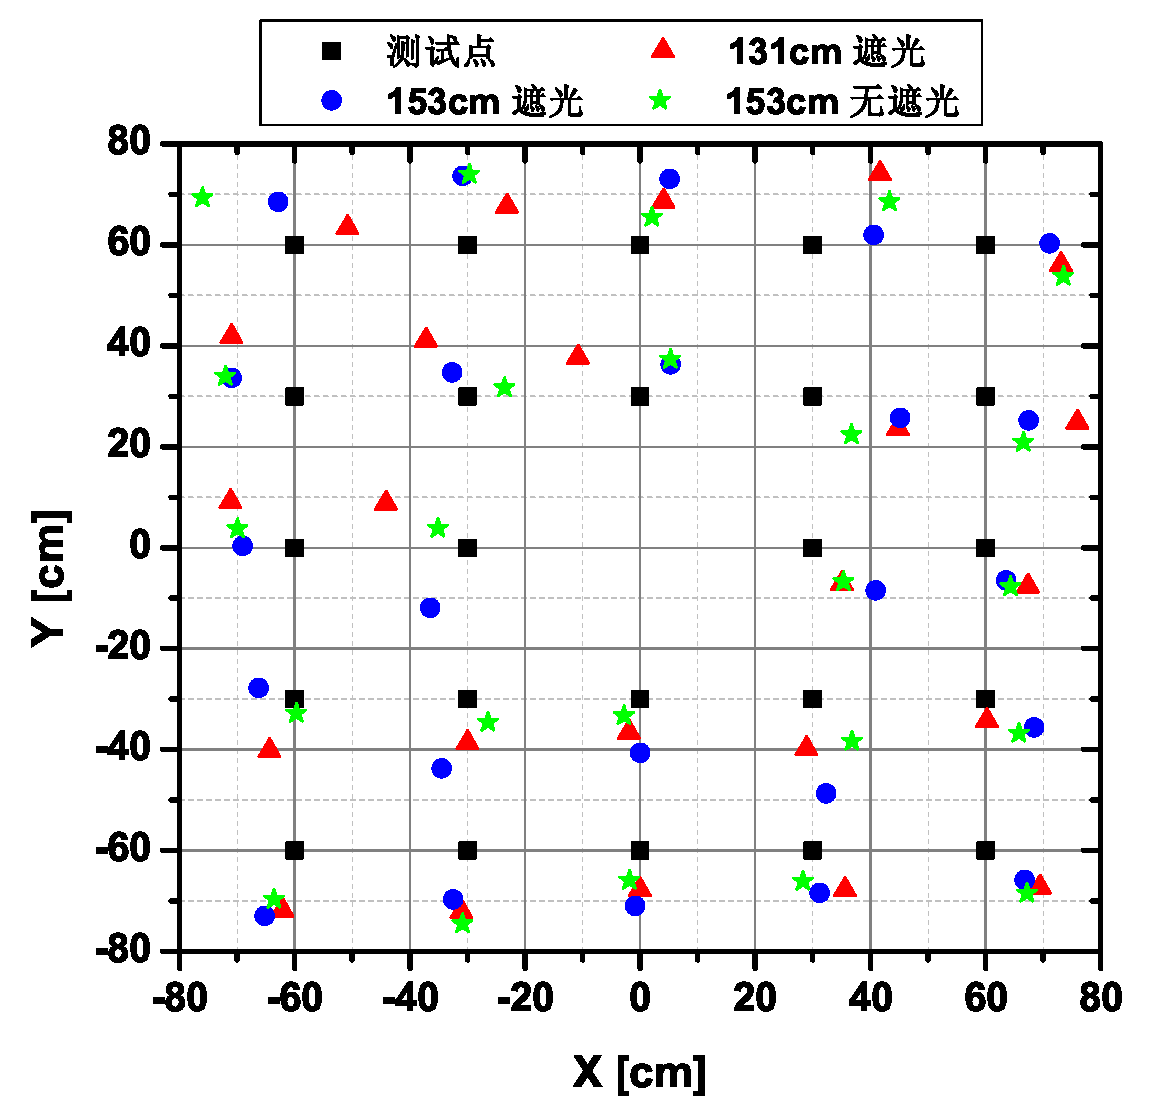
\includegraphics[width=0.7\linewidth]{FIG/5-8.eps}
                \caption{不同环境下的NLOS VLP系统2D性能}
                \label{fig:errors-2D}
\end{figure}


     \begin{figure}[!t]
                \centering
                \begin{minipage}{0.45\linewidth}
                  \centering
                  \centerline{\includegraphics[width=\textwidth]{FIG/fig12a.pdf}}
                  \centerline{(a)}
                \end{minipage}
                \begin{minipage}{0.45\linewidth}
                  \centering
                  \centerline{\includegraphics[width=\textwidth]{FIG/fig12b.pdf}}
                  \centerline{(b)}
                \end{minipage}\\
                \begin{minipage}{0.5\linewidth}
                  \centering
                  \centerline{\includegraphics[width=\textwidth]{FIG/fig12c.pdf}}
                  \centerline{(c)}
                \end{minipage}
                \vfill
                \caption{NLOS VLP的3D定位性能: (a) 131 cm遮光; (b) 153 cm遮光; (c) 153 cm有环境光.}
                \label{fig:errors-3D}
 \end{figure}

因此,本系统分析了实验结果中的误差。在方程组(\ref{mx:world-ccww})中,由于$\mathbf{R}$实际上是已知的,为了忽略$\mathbf{R}$的影响,假设$\mathbf{R}$是单位矩阵,这样目标向量$-\mathbf{R}^{-1} \mathbf{t} $的误差分析就可以转化为$\mathbf{t}$的分析,现在,$(x_w,y_w,z_w )^T$是已知的。因此,改变$\mathbf{t}$与改变$(x_c,y_c,z_c)$是等价的。因此,将方程(\ref{mx:cemara-xycc})的左右两边都除以$z_c$并代入方程(\ref{mx:pixel-uvxy})中,并经过变形,得到:
    \begin{equation}\label{eq:u-u0}
                \frac{f_{0}x_{c}}{z_{c}}=\frac{f_{0}x_{c}}{z_{c}^{'}+\Delta z_{c}}=u-u_{0}=u^{'}+\Delta u-u_{0},
    \end{equation}
其中 $f_0=f/dx$,$\Delta u$ 是 $u$ 的估计误差,$\Delta z_c$ 是 $z_c$ 的估计误差,它是 函数(\ref{mx:world-ccww}) 和 (\ref{mx:reprojection}) 中的一个独立变量,因此 $x_c$ 将被视为 $z_c$ 的隐函数,而观察到的误差是由于 $z_c$引起的。公式(\ref{eq:u-u0}) 是一个理想的情况,而实际的计算过程如下:
     \begin{equation}\label{eq:u'-u0}
                \frac{f_{0}x_{c}}{z_{c}^{'}}=u^{'}-u_{0}.
  \end{equation}
 现在假设:
     \begin{equation}\label{eq:delta u}
        \Delta u= \eta (u^{'}-u_{0}),
    \end{equation}   
$\Delta z_{c}$可以表示为:
     \begin{equation}\label{eq:delta zc}
    \Delta z_{c}=\eta z_{c}.
\end{equation}
在实验中,$z_{c}=153$,所以,$\Delta z_c=153 \eta$。如果 $x_c$ 被视为函数(\ref{mx:world-ccww}) 和 (\ref{mx:reprojection}) 中的一个独立变量,那么 $z_c$ 可以被视为 $x_c$ 的隐函数。$x_c$ 的估计误差的最大值是 $ \Delta x_c \approx60 \eta$。相同的 $u$ 误差对 $x_c$ 和 $z_c$ 有完全不同的影响,因此也对 $y_c$ 有影响。另外,$\eta \approx 1$ 或者甚至 $\eta>1$ 可能对 $(u-u_0)\propto 0$ 成立,这会使得 $ \Delta z_c$ 倍增。换句话说,当手机放置在LED正下方时,将观察到最大的定位误差。这就是不计算中心点误差的原因。在这种情况下,当高亮点接近图像中心时,相机位置被认为是直接在LED下方。另外,在仔细分析图 \ref{fig:errors-3D} 中的误差分布时,可以观察到最大的误差集中在第二象限,这里靠近窗户,室外直射光对这个区域有很大的影响。通过图 \ref{fig:errors-3D}可以得出结论:环境光引起的干扰比传输距离对z轴定位精度的影响更严重。

 \begin{figure}[!t]
                \centering
                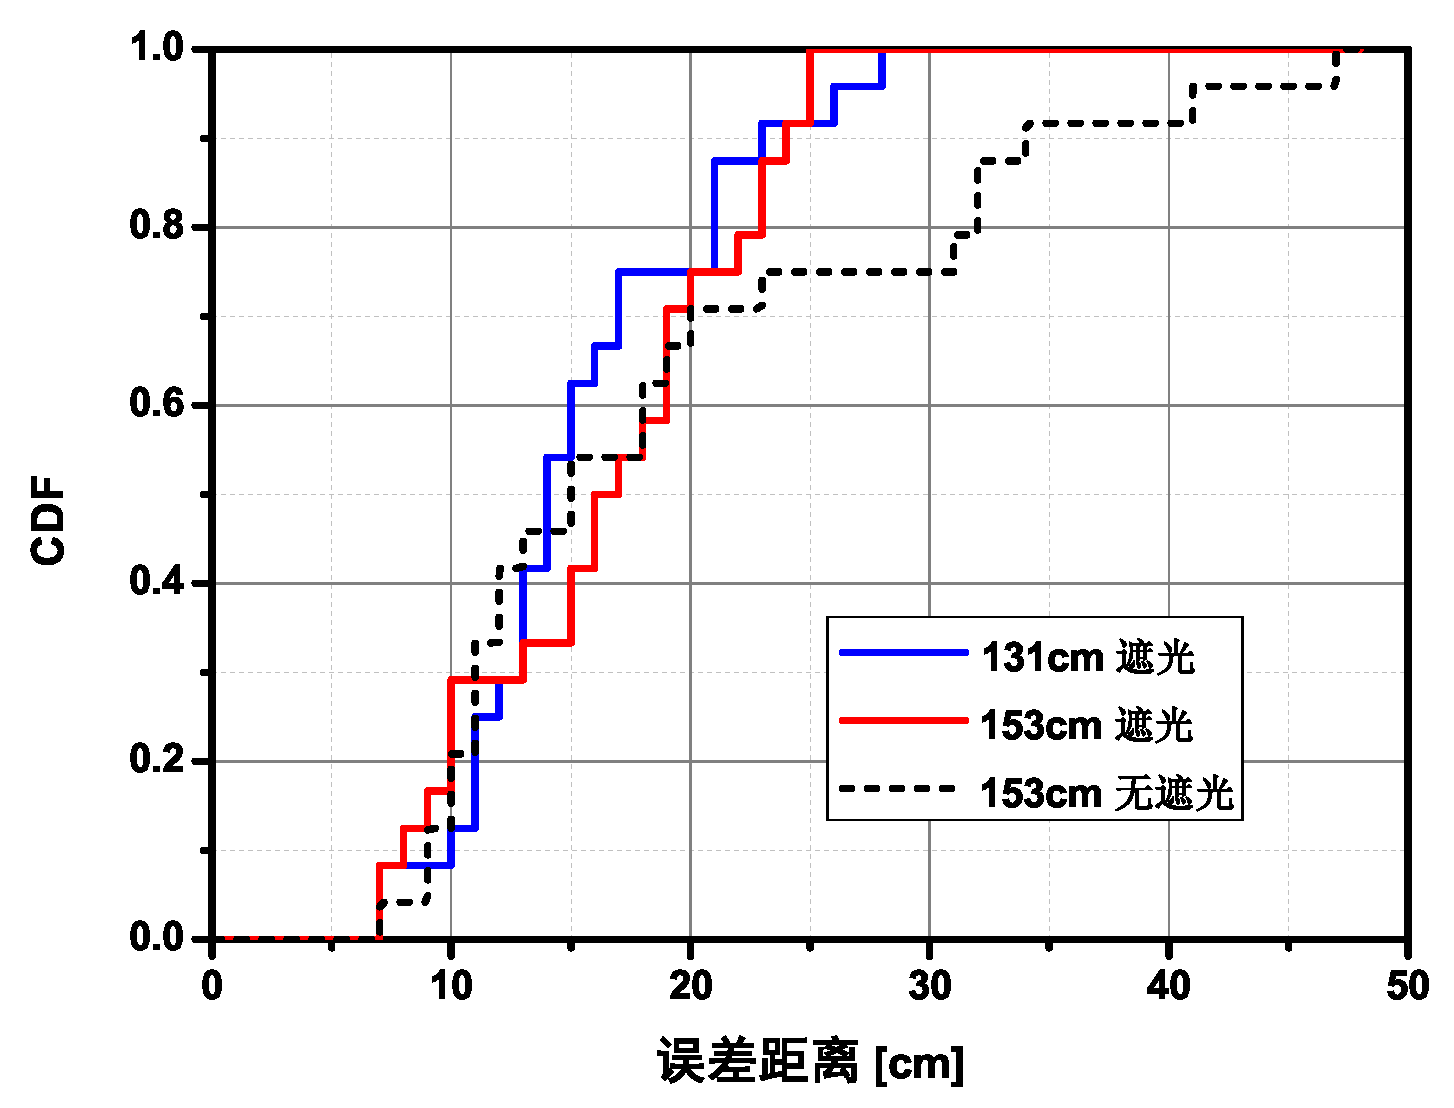
\includegraphics[width=0.7\linewidth]{FIG/5-10.eps}
                \caption{不同条件下的CDF对比}
                \label{fig:cdf}
 \end{figure}

接下来,系统确定了三种情况误差的累积分布函数(Cumulative Distribution Function, CDF),如图 \ref{fig:cdf} 所示。在没有环境光的情况下,CDF曲线几乎相同,而在有环境光的情况下则不是这样,说明环境光比距离的增加对系统性能影响更大。注意,在没有环境光干扰的情况下,所提出的系统可以实现在置信度90$\%$的情况下精度小于22 cm的3D定位,而在有环境光的情况下,这一数字增加到34 cm。显然,系统误差的最大值增加了很多,大于45 cm,反映了在环境光干扰下系统性能严重衰减。

表 \ref{tab:VLP systems} 显示了VLP最新的研究成果。与文献 \parencite{vlp-yang2019visible} 报道的唯一一项NLOS IS-VLP系统研究结果相比,该系统在置信度为90$\%$下的精度为75 cm,很难达到IPS的要求,此外,该系统还需要IMU的辅助。因此,本文所提出的系统更简单、更准确。此外,本文还利用LDM模型计算了反射光产生的IS亮度,为亮度提供了直观的数学表达式。

与LOS VLP相比,所提出的系统克服了LOS链路阴影或遮挡带来的挑战。同时,在仅需要单个IS和LED基础上,通过两个虚拟LED设计实现性能提升。然而,与表 \ref{tab:VLP systems} 中文献 \parencite{vlcp-jin2022adaptive} 和文献 \parencite{vlp-bai2021computer} 的LOS VLP系统相比,所提出的系统性能较差。这是因为硬件系统过于简单和NLOS链路的影响,所提出的NLOS IS-VLP定位精度有限。此外,所提出的3D NLOS IS-VLP算法必须要求相机总是可以捕捉到两个高亮点,由于其中一个是由LED在地板上的投影点形成的,由于LED是固定的,所以它的位置也是固定的。因此,LED在地板上的投影点必须始终在相机的视野内,这大大限制了系统可用的定位范围。考虑到所提出系统性能和定位范围有限,本系统未来还需要进一步改进和优化。
\begin{table}[!t]
                \centering  
                \caption{不同方案的性能比较}  
                \label{tab:VLP systems}  
                \begin{tabular}{lccccc}  
                  \toprule 
                \makebox[0.1\linewidth][l]{$\textbf{方案}$} &\makebox[0.1\linewidth][c]{$\textbf{LED数量}$}&\makebox[0.15\linewidth][c]{$\textbf{接收端类型}$}&\makebox[0.1\linewidth][c]{$\textbf{信道}$}&\makebox[0.2\linewidth][c]{$\textbf{90$\%$置信度的精度}$}&\makebox[0.15\linewidth][c]{$\textbf{辅助传感器}$}\\ 
                \midrule  
                  \parencite{vlcp-jin2022adaptive}&1&5 PDs&LOS&$<$6 cm&No  \\
                  \parencite{vlp-bai2021computer}&4&1 IS&LOS&$<$4.6 cm&No  \\
                  \parencite{vlp-yang2019visible}&1&1 IS&NLOS&75 cm&Yes  \\
                  Ours&1&1 IS&NLOS&$<$22 cm&No  \\
                  \bottomrule 
                \end{tabular}
\end{table}



\section{本章小结}
 本章主要介绍了基于亮度分布模型NLOS IS-VLP系统的基本原理和工作流程以及最后的性能测试。首先,本章提出了一种亮度分布模型,它可以用来表示一次反射光在图像传感器上的亮度分布情况。利用这种亮度分布模型,可以证明在仅有一个LED时,图像传感器上捕捉到的两个高光点可以被视为是两个虚拟的LED通过LOS在图像传感器上面的投影。其中,这两个虚拟LED的位置被证明是LED在反射面的投影和关于反射面的对称点。在通过第三章的NLOS OCC系统得到LED的坐标和高光点的像素坐标之后,可以构建基于两个虚拟LED的LOS IS-VLP系统,利用第二章给出的基于计算机视觉的重投影误差最小化算法实现的接收端的位置估计。从结果可以得知所提出的NLOS IS-VLP系统方案在只有一个LED的情况下能够利用反射光实现3D VLP,成功的克服了本文开篇提出的VLP系统面临的两个主要难点。但是,从系统的定位精度来看,通过反射光进行NLOS IS-VLP的性能还有待提高。
    \chapter{基于双目立体视觉的NLOS IS-VLP系统}
\section{系统概述}
本章在前一章的基础上,通过对硬件系统进行改进,设计了一个基于双目立体视觉的NLOS IS-VLP系统,并且给出了系统流程、实验设计以及性能测试。首先,由于双目立体视觉算法可以实现在已知一个点在左右目图像上的像素坐标的情况下,可以计算其在相机坐标系的坐标。因此,本系统通过双目相机只需要捕获LED关于地面的对称点来进行VLP。在惯性测量单元(IMU)的辅助下又可以获得相机的姿态,通过计算机视觉算法很容易实现基于单灯的NLOS IS-VLP系统。

\section{双目立体视觉算法}
本方案利用双目相机实现单点定位,在只需要一个LED的情况下可以实现3D定位。本文将在这里给出基于双目立体视觉算法的定位原理。已知空间中一点在左目右目相机上的投影点的像素坐标,双目立体视觉算法可以用来计算空间中的这一点在左目或者右目相机坐标系CCS中的3D坐标。假设,空间中的一点$P$在左目和右目CCS中的坐标分别是$\mathbf{P_{l}}$ 和 $\mathbf{P_{r}}$,如图所示,它们之间的关系由下式给出:
\begin{equation}\label{Pl=RPr+T}
\mathbf{P_{l}=RP_{r}+T}
\end{equation}
其中, $\mathbf{R}$ 和 $\mathbf{T}$分别是右目相机相对于左目相机的旋转矩阵和平移向量,它们的值可以通过对双目相机标定得到。假设$P$点在左目和右目相机照片上的投影点为$P_{1}$ 和 $P_{2}$,它们的值为($u_{1}$, $v_{1}$)和 ($u_{2}$, $v_{2}$)。用${z_{l}}$ 和 ${z_{r}}$分别表示$\mathbf{P_{l}}$ 和 $\mathbf{P_{r}}$的Z轴坐标,像素坐标系PCS和CCS之间存在关系入下:
\begin{equation}\label{zlzruv}
\begin{cases} 
  z_{l}\mathbf{t_{1}=K_{l}P_{l}}  \\
  z_{r}\mathbf{t_{2}=K_{r}P_{r}}                      
\end{cases}
\end{equation}
其中,$\mathbf{t_{1}}$=($u_{1}$, $v_{1}$,1),$\mathbf{t_{2}}$=($u_{2}$, $v_{2}$,1);$\mathbf{K_{l}}$ 和 $\mathbf{K_{r}}$分别是左目和右目相机的内参矩阵。通过求解方程(\ref{Pl=RPr+T})和 (\ref{zlzruv}),可以计算出$\mathbf{P_{l}}$的值。
\begin{figure*}[!htbp]
  \centering
  \includegraphics[width=0.8\linewidth]{FIG/dualcamera.pdf}
 \caption{双目立体视觉模型}
\label{fig:dualcamera}
\end{figure*}
可以建立关于点$P$从世界坐标系WCS到左目CCS的转换关系:
\begin{equation}\label{PlPw}
\mathbf{P_{l}=R_{l}P_{w}+T_{l}}
\end{equation}
其中,$\mathbf{R_{l}}$ 和 $\mathbf{T_{l}}$分别是WCS相对于左目CCS的旋转矩阵和平移向量。由此,可以得到左目相机的焦点在WCS中的位置:
\begin{equation}\label{wl}
\mathbf{W_{l}=-R_{l}^{-1}T_{l}}
\end{equation}
注意,左目相机的焦点在WCS中的位置也就是本系统的目标位置。

在 方程(\ref{PlPw})和(\ref{wl})中$\mathbf{R_{l}}$的值可以通过一个惯性测量单元IMU测量得到,由此,通过方程(\ref{PlPw})可以计算出$\mathbf{T_{l}}$。然后再代入到方程(\ref{wl})中,目标位置即可求解。在多数情况下,由于相机参数误差、系统测量误差和PCS中投影坐标的估计误差,方程组(\ref{Pl=RPr+T})和 (\ref{zlzruv})可能没有实数解。因此,在这项工作中,本系统将解方程组 (\ref{Pl=RPr+T})和 (\ref{zlzruv})转换成找$P_{1}$ 和 $P_{2}$的重投影误差的最小值。对于2D重投影误差函数,存在一个求解最小值点的最优解,其给出为:
\begin{equation}\label{pl^*}
\mathbf{P_{l}}^\ast = \arg\min _{\mathbf{P_{l}}} \left \{ 
\begin{Vmatrix}
\mathbf{t_{1}-K_{l}P_{l}}/z_{l}
\end{Vmatrix}^{2}
+
\begin{Vmatrix}
\mathbf{t_{2}-K_{r}R^{-1}(P_{l}-T)}/z_{r}
\end{Vmatrix}^{2}
\right \} 
\end{equation}
最后,可以获得相应的目标位置表达式,如下所示:
\begin{equation}\label{wl*}
\mathbf{W_{l}^{*}=P_{w}-R_{l}^{-1}P_{l}^{*}}
\end{equation}

\section{误差补偿算法}
\begin{figure}[!t]
\begin{minipage}{0.49\linewidth}
  \centerline{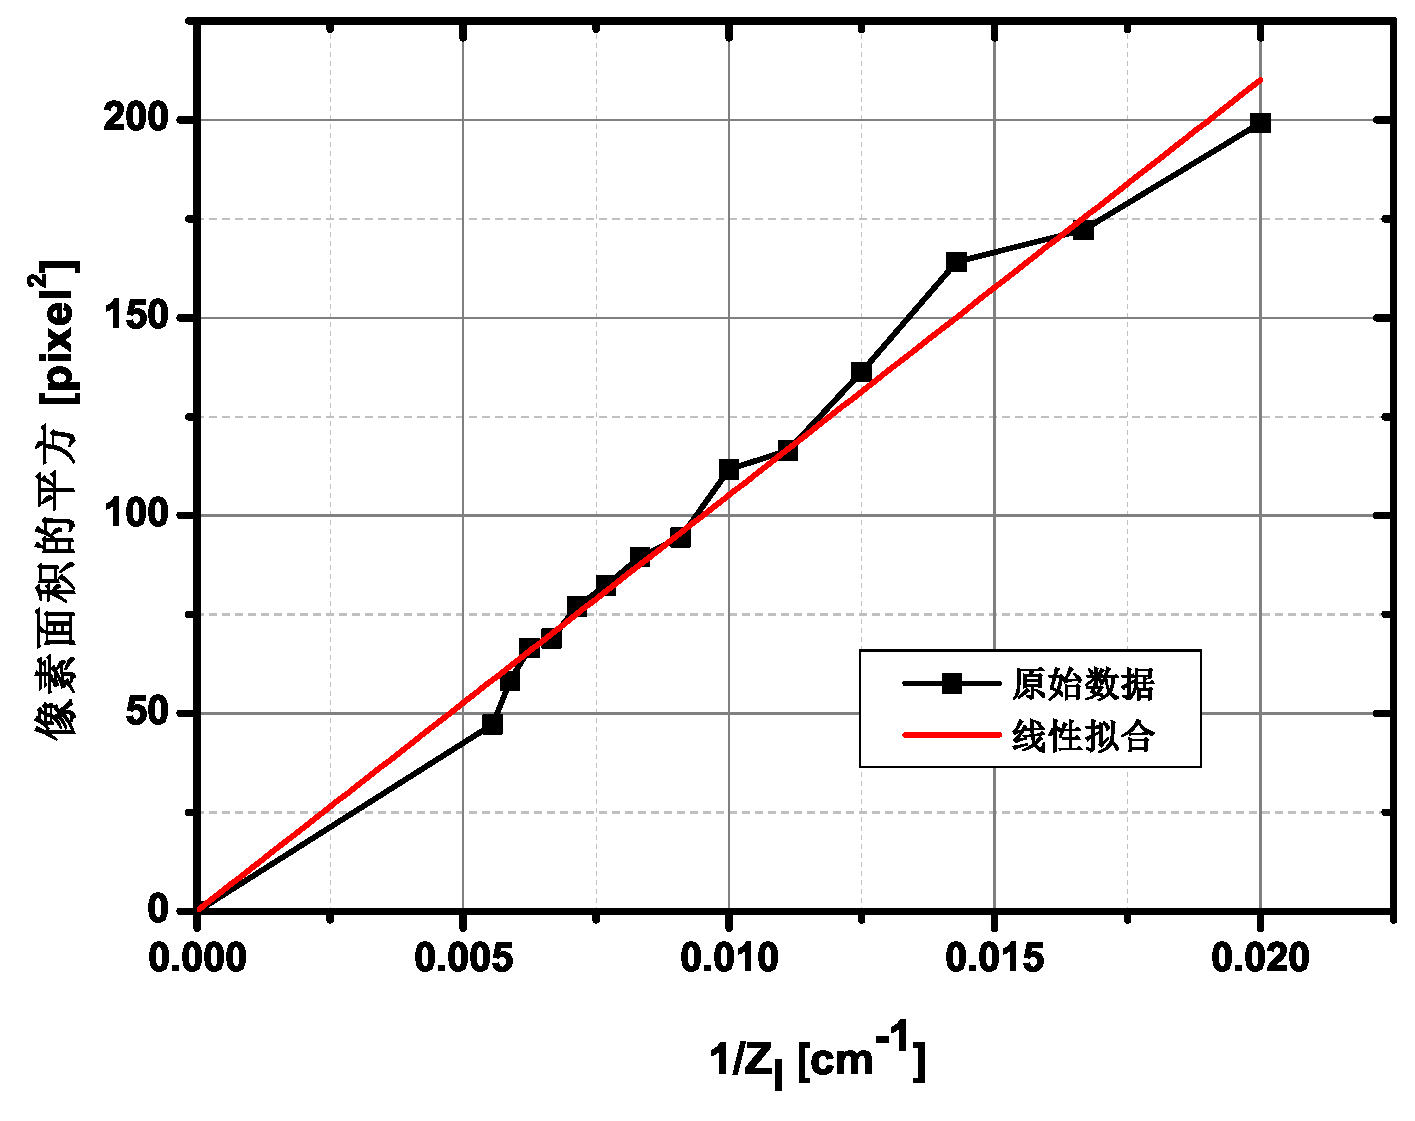
\includegraphics[width=\textwidth]{FIG/5-12b.eps}}
  \centerline{(a)}
\end{minipage}
\hfill
\begin{minipage}{0.49\linewidth}
  \centerline{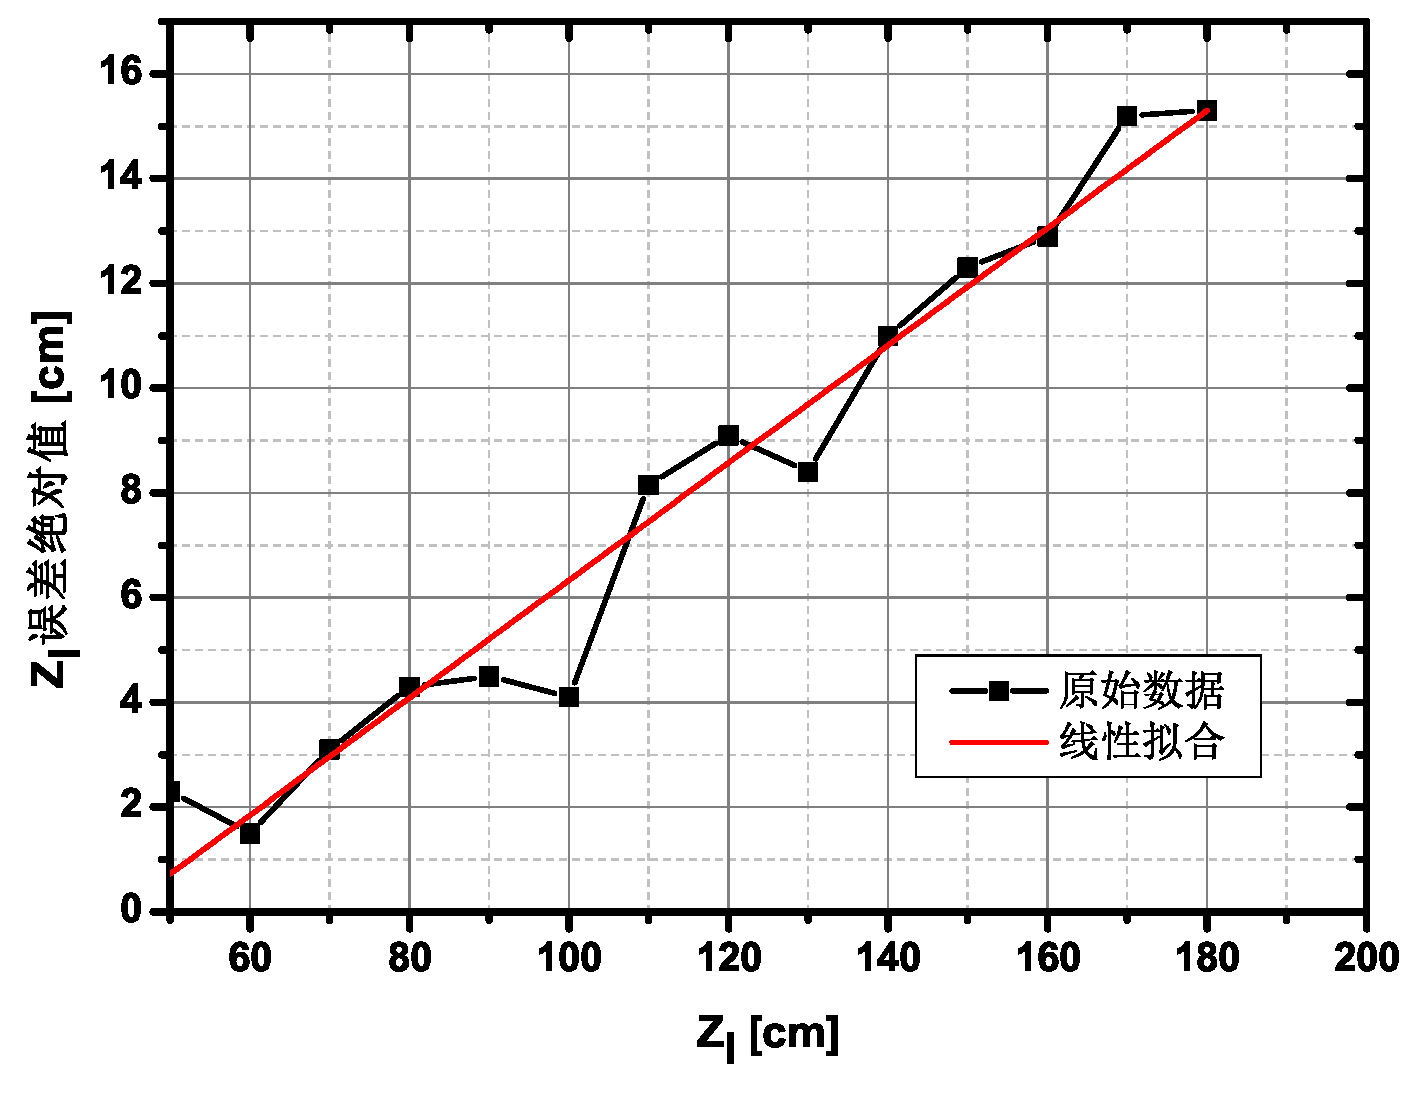
\includegraphics[width=\textwidth]{FIG/5-12a.eps}}
  \centerline{(b)}
\end{minipage}
\vfill
\caption{误差分析: (a)对称点附近高亮区域面积的平方和$z_{l}$倒数的线性拟合,(b)$z_{l}$误差绝对值与$z_{l}$}
\label{fig:erroranlysiszw}
\end{figure}
从公式(\ref{pl^*})和(\ref{wl*})可以看出,系统误差有三个主要来源,分别是相机参数、IMU角度估计和PCS上对称点的估计误差。为了简化误差分析,本系统暂不考虑来自相机参数和IMU角度估计的系统误差部分,只关注对称点的估计误差对系统性能的影响,并提出了一个误差补偿算法来补偿它。因此,本系统首先通过公式(\ref{pl^*})和(\ref{wl*})给出系统误差函数,如下所示:
\begin{equation}\label{delta wl*}
\Delta\mathbf{ W_{l}=W_{l}^{*}-W_{l}^{'}=R_{l}^{-1}(P_{l}^{'}-P_{l}^{*})=R_{l}^{-1}}\Delta \mathbf{P_{l}}
\end{equation}
其中$\Delta\mathbf{ W_{l}}$是系统误差,包括$x$、$y$和$z$轴上的估计误差,$\mathbf{W_{l}{'}}$是所提出的系统的估计值。$\mathbf{P_{l}{'}}$和$\Delta\mathbf{ P_{l}}$分别是点$P$在左相机CCS上的估计值和估计误差。由于忽略了IMU角度估计误差,等式(\ref{delta wl*})中的$\mathbf{R_{l}}$的值可以确定。大量研究工作表明,在$\Delta\mathbf{ P_{l}}$中, $z $ 轴上的估计误差比 $ x $ 和 $ y $ 轴上的大得多,这也与实验中的结果一致。因此,我们认为 $ z_ { l } $ 的估计误差是影响系统误差的最重要因素。因此,我们设计了一个针对双目视觉的NLOS IS-VLP系统的误差补偿(Error Compensation, EC)算法,通过优化 $ z_ { l } $ 来补偿 $ z $ 轴上的系统误差。在EC中,我们只讨论了 $ z_ { l } $ 的误差。将公式(\ref{Pl=RPr+T})和(\ref{zlzruv})展开成方程形式,可以将 $ z_ { l } $ 表示为:   
\begin{equation}\label{xlylzl}
  {z_{l}=f_{lx}f_{rx}t_{0}/(f_{rx}(u_{1}-u_{l})-f_{lx}(u_{2}-u_{r}))}	
\end{equation}
其中$u_{l}$是左相机焦点在PCS上的投影的横坐标,$f_{lx}$是左相机的焦距与每个像素长度的比值,$u_{r}$,$f_{rx}$类似。我们选择$z_{l}^{'}$作为$z_{l}$的测量值,$\Delta z_{l}$被视为$z_{l}$的误差,表示为:
\begin{equation}\label{xl'yl'zl'}
  \Delta z_{l}=z_{l}-z_{l}^{'}= z_{l}z_{l}^{'}(f_{lx}\Delta u_{2}-f_{rx}\Delta u_{1})/ f_{lx}f_{rx}t_{0}
\end{equation}
其中$\Delta u_{1}$和$\Delta u_{2}$分别是$u_{1}$和$u_{2}$的估计误差。显然,PCS上对称点周围高亮区域的像素面积大小会随着$z_{l}$的增加而减小。这一点在图\ref{fig:erroranlysiszw}(a)中得到了实验验证。注意,根据相对误差的一致性,可以认为$\Delta u_{1}$、$\Delta u_{2}$和$z_{l}$之间存在反比关系。通过这种关系,$\Delta z_{l}$在公式(\ref{xl'yl'zl'})下与$z_{l}^{'}$呈线性关系。
 
本系统建立了一个实验测试平台,其中LED固定在距离地面40 cm的高度,相机朝向LED的反射点,以确保$\mathbf{R_{l}}$是单位矩阵,消除了IMU角度估计误差的影响。图\ref{fig:erroranlysiszw}(b)显示了$\Delta z_{l}$与$z_{l}$之间的绝对值的测量数据点和线性拟合,它们是线性关系。注意,得到的结果受到相机灵敏度和地板平整度的影响。相机ISO设置为50,以确保可以捕捉和检测到LED边缘。考虑到线性效应不明显,$z$轴上的误差随着相机到LED对称点的距离的增加而增加。因此,为了补偿误差,使用线性拟合的系数$\lambda=0.112$,如下所示:
 \begin{equation}\label{ECzl}
 {z_{l}^{*}=z_{l}^{'}(1+\sigma \lambda/(1-\lambda ) ) }
\end{equation}
其中,$\sigma$的取值只能是“1”或者“0”,它被用来决定$z_{l}$的测量值是否需要被优化。

EC算法的实现流程如图\ref{fig:EC-BPE}所示,其中$H$是PCS上对称点周围的高亮区域。假设$\sigma=1$,可以通过公式(\ref{zlzruv})计算$(u_{1},v_{1})$和$(u_{2},v_{2})$,然后由公式(\ref{ECzl})计算$z_{l}=z_{l}^{*}$。注意,($i $)如果两者都在对称点周围的高亮区域内,则$\sigma=1$,否则$\sigma=0$;($ii $)确定了$\sigma$后,可以优化$z_{l}$;以及($iii $)然后,通过将其代入公式(\ref{wl})来确定EC算法下的目标值。
\begin{figure}[!t]
\centering\includegraphics[width=\textwidth]{FIG/EC procedure.pdf}
\caption{EC算法流程图}
\label{fig:EC-BPE}
\end{figure}





\section{系统方案}

所提出方案的系统模型如图\ref{fig:dualcam_systemscheme}所示,主要由NLOS OCC子系统和基于双目立体视觉的单点定位子系统组成,其中NLOS OCC系统的实验过程在第三章已经详述,通过它来实现对LED坐标的提取。对于位置估计子系统,本系统提出了两种不同的方案,都是在只有一个LED的情况下实现3D NLOS IS-VLP。第一种是将LED在地面上的对称点视为点$P$来估计相机位置。这种方案系统性能会随着地面粗糙度的增加而降低。当粗糙程度过大时,图像检测高光亮点可能失败。为了克服这个问题,本系统提出了一种地标增强(Label Enhanced, LBE)的可见光成像定位方案(LBE IS-VLP),将方案一中的点$P$替换为标签,该标签是LED在反射表面上的正投影,需要提前标记。与NLOS IS-VLP通过像素灰度值检测高亮区域相比,LBE IS-VLP通过标签的形状来识别标签,因此粗糙反射面对其影响较小。
\begin{figure*}[!t]
  \centering
  \includegraphics[width=0.85\linewidth]{FIG/systemscheme.pdf}
 \caption{基于双目相机的NLOS IS-VLP系统模型}
\label{fig:dualcam_systemscheme}
\end{figure*}

第一种方案,在发射端LED光信号进行调制;在接收端双目相机通过切换长短曝光来实现通信和捕捉反射面的高光点。在通过NLOS OCC子系统获取到LED的坐标之后,很容易得到LED关于地面对称点的坐标即(${x_{0}}$,${y_{0}}$,$-z_{0}$),由于LED通过NLOS链路在左右摄像机上的投影等于对称点通过LOS链路的投影。将此对称点的坐标和其在左右目相机上的投影点坐标代入到双目立体视觉算法中,就可以计算出目标位置。通过边缘检测和椭圆拟合,可以得到此坐标。如图\ref{fig:dual_imageprocessing}(a)所示,可以将拟合椭圆的中心点坐标作为对称点在左右目相机上的投影点坐标。
\begin{figure*}[!htbp]
\begin{minipage}{0.75\linewidth}
  \centerline{\includegraphics[width=\textwidth]{FIG/imageprocessing.pdf}}
  \centerline{(a)}
  \label{fig:imageprocessing-a}
\end{minipage}
\hfill
\begin{minipage}{0.23\linewidth}
  \centerline{\includegraphics[width=\textwidth]{FIG/cornerdetecting.pdf}}
  \centerline{(b)}
  \label{fig:imageprocessing-b}
\end{minipage}
\vfill
\caption{参考点坐标提取: (a) 椭圆拟合提取高光点坐标;(b) 角点检测标签位置}
\label{fig:dual_imageprocessing}
\end{figure*}


LBE IS-VLP方案基本上与NLOS IS-VLP相同,只是将双目视觉算法中的点$P$替换为标签,该标签是LED在反射面上的正投影,在实验之前进行标记。因此,在LBE IS-VLP中,可以根据LED坐标计算标签在世界坐标系上的坐标。与NLOS IS-VLP一样,也可以使用NLOS OCC子系统接收LED坐标。同时,可以使用双目相机来识别标签。这种方案涉及的详细过程与NLOS IS-VLP非常相似,只是将标签视为参考点。标签的世界坐标系下的坐标由标签和LED之间的几何关系确定,即(${x_{0}}$, ${y_{0}}$,${0}$)。本方案使用了角点检测方法来处理来自左右相机的照片,从而检测标签,标签在像素坐标系上的坐标是四个角点坐标的平均值,见图\ref{fig:dual_imageprocessing}(b)。
 
\section{实验与性能}
\subsection{实验环境}
所提出的系统的实验测试平台如图\ref{fig:dual_environment-setup}所示。发射端由工作频率为3.3 kHz的STM32微控制器单元、驱动模块和LED组成,LED位于距地面1.96 m的高度,其在地面上投影点是WCS的原点。在接收端,使用ZED2双目相机捕捉左右相机的两幅图像,而IMU用于测量相机姿态。首先,本系统校准了ZED2以获得其两个相机的内部参数矩阵。经过内参标定,发现两个相机之间的旋转矩阵基本上近似是一个单位矩阵,相机之间只在x轴有位移。
\begin{figure}[!htbp]
\centering\includegraphics[width=0.7\textwidth]{FIG/experimentsetup.pdf}
\caption{实验硬件系统}
\label{fig:dual_environment-setup}
\end{figure}


因此,在(\ref{Pl=RPr+T})中有$\mathbf{R=I}$和$\mathbf{T}=[t_{0},0,0]$,其中$t_{0}$是一个常数。注意,对于每个实验,本系统都调整了ZED2的位置,以确保它在地板上的投影的位置与一个测试点重合。本系统测量了ZED的高度作为测试点z轴坐标。通过比较测试点的坐标和使用所提出的系统估计的ZED2的坐标,确定了系统误差。本系统对总共60个点进行了这样的操作并估计了RMSE和误差CDF。所有使用的关键系统参数都给出在表\ref{tab:dual_parameter}中。
\begin{table}[!htbp]
	\centering  
	\caption{基于双目视觉的NLOS VLP系统实验参数}  
	\label{tab:dual_parameter}   
	\begin{tabular}{lc}  
        \toprule
        \makebox[0.35\linewidth][l]{$\textbf{实验参数}$} &\makebox[0.5\linewidth][c]{$\textbf{参数值}$}\\ 
        \midrule
		测试环境& 200 $\times$ 200 $\times$ 196 $\mathrm{cm^{3}}$ \\
		MCU 输出频率& 3.3 kHz \\
		LED 输出功率&1.4 W\\
		LED 工作电压&5 V\\
		LED 坐标&(0,0,196) \\ 
		Label 坐标&(0,0,0) \\ 
		IMU 自由度&9 \\
		双目相机尺寸&3840 $\times$ 1080 \\
		双目相机相对位置&(12,0,0)  \\
		\bottomrule
	\end{tabular}
\end{table}

\subsection{系统性能}
通过所提出的系统的估计值和测量值之间的差的绝对值,确定了60个数据集的3D平均定位误差和RMSE。实验结果如表\ref{tab:systemerror}所示,其中最低的3D平均误差和RMSE分别为37.2和44.6 cm。此外,我们还计算了60个数据集的X、Y和Z轴上的平均误差,分别为6.96、6.01和35.32 cm。
  \begin{table}[!htbp]
                \centering  
                \caption{各种方案的性能比较}  
	\label{tab:systemerror}   
                \begin{tabular}{lccccc}  
                  \toprule 
                \makebox[0.15\linewidth][l]{$\textbf{方案}$} &\makebox[0.1\linewidth][c]{$\textbf{X (cm)}$}&\makebox[0.1\linewidth][c]{$\textbf{Y (cm)}$}&\makebox[0.1\linewidth][c]{$\textbf{Z (cm)}$}&\makebox[0.15\linewidth][c]{$\textbf{平均误差 (cm)}$}&\makebox[0.15\linewidth][c]{$\textbf{RMSE (cm)}$}\\ 
                \midrule  
                  NLOS IS-VLP &6.96&6.01&35.32&37.27&44.59 \\
		EC NLOS IS-VLP&6.96&6.01&22.58&26.10&31.02 \\ 
		LBE IS-VLP &3.62&3.24&4.50&7.31&7.74 \\
                  \bottomrule 
                \end{tabular}
\end{table}


图\ref{fig:2Derrorcompensation}描绘了NLOS IS-VLP在X-Y平面上的2D定位性能,从中可以看出,NLOS IS-VLP系统对于X-Y平面上的性能总体较好,除了一些远离LED的测试点有较大的偏差。图\ref{fig:NLOS VLP system error}显示了X、Y和Z轴以及3D的CDF图。 X 和 Y 轴上的CDF与图\ref{fig:2Derrorcompensation}的结果基本上一致,可以实现在90$\%$的置信度下小于 15 cm的定位精度。


\begin{figure}[!htbp]
\centering\includegraphics[width=0.65\textwidth]{FIG/2derror2.eps}
\caption{各种方案2D误差对比}
\label{fig:2Derrorcompensation}
\end{figure}

\begin{figure}[!htbp]
\centering\includegraphics[width=0.65\textwidth]{FIG/517-b.eps}
\caption{NLOS IS-VLP系统X、Y和Z轴以及3D的CDF}
\label{fig:NLOS VLP system error}
\end{figure}


然而,对于 Z 轴和 3D的 CDF来说,在80$\%$的置信度下小于60 cm的定位精度并不令人满意。与没有经过误差补偿的NLOS IS-VLP相比,经过误差补偿的NLOS IS-VLP系统的最低平均误差和 RMSE 值分别降低至 26.10 和 31.02 cm。注意,在90$\%$的置信度下3D定位误差已经降到50 cm, 此外, CDF 曲线显示了误差补偿算法的效果,见图 \ref{fig:errorcompensation}。
\begin{figure}[!t]
\centering\includegraphics[width=0.65\textwidth]{FIG/518.eps}
\caption{有无误差补偿的CDF对比}
\label{fig:errorcompensation}
\end{figure}

\begin{figure}[!t]
\centering\includegraphics[width=0.65\textwidth]{FIG/519.eps}
\caption{LBE VLP方案:X、Y和Z轴以及3D的CDF}
\label{fig:cdflabel}
\end{figure}


同样的,系统对LBE IS-VLP方案进行了测试、测量和性能评估,与NLOS IS-VLP相同,估计了60组数据的RMSE和平均定位误差。实验结果如表\ref{tab:systemerror}所示,其中最低平均误差和RMSE分别为7.31和7.74 cm;X、Y和Z轴上的平均误差分别为3.62、3.24和4.50 cm。图\ref{fig:cdflabel}显示了X、Y和Z轴以及3D的CDF图,其中X、Y和Z轴都可以实现在90$\%$的置信度下小于8 cm的精度,而3D的性能可以实现在90$\%$的置信度下小于11 cm的精度。



\begin{figure}[!t]
\centering\includegraphics[width=0.65\textwidth]{FIG/520b.eps}
\caption{几种方案Z轴以及3D的CDF比较}
\label{fig:comparation}
\end{figure}


与NLOS IS-VLP相比,LBE IS-VLP在X-Y平面上距离LED较远的测试点明显提高了性能,见图\ref{fig:2Derrorcompensation}。图\ref{fig:comparation}描绘了LBE IS-VLP、NLOS IS-VLP和带有EC算法的NLOS IS-VLP几种方案下X、Y和Z轴以及3D的CDF性能。LBE IS-VLP具有参考点(标签或对称点)在像素坐标系上的估计误差较小,以及在相机坐标系上的估计误差较小,因为对称点到相机的距离比标签到相机的距离大得多。因此,从图\ref{fig:comparation}可以明显看出,与NLOS IS-VLP相比,LBE IS-VLP方案具有最佳性能。
 
 与LOS VLP相比,所提出的系统克服了LOS链路阴影或遮挡以及LED数量的限制,在仅有一个LED的情况下可以实现较高精度的定位。与所提出的基于亮度分布模型的NLOS VLP系统相比,通过改进接收端可以提高NLOS VLP系统的性能。



\section{本章小结}
 本章所提出的基于双目立体视觉的NLOS IS-VLP系统是在前一章的基础上,通过对硬件系统以及实验方案进行改进,来提高系统性能的。首先,本章介绍了基于双目立体视觉的定位算法,通过对误差进行分析给出了一个误差补偿算法。在此之后,给出了两种试验方案,以及实验测试了它们各自的性能。虽然,本文所提出的NLOS IS-VLP可以实现任意姿态的3D定位,但是定位性能依旧有待提高,虽然通过误差补偿,系统性能有所提高,但是,跟LBE IS-VLP方案相比,性能差距明显。然而,LBE IS-VLP方案需要提前进行标签的标注。总的来说,本系统成功的克服了本文开篇提出的VLP系统面临的两个主要难点,并且得到了一个较为可观的性能。
    
	% 自行根据需要添加章节。

	\backmatter %章节不编号但页码继续
	%%%%%%%%%%%%%%%%%%%%%%%%%%%%%%%%%%%%%%%%%%%%%%%%%%%%%%%%%%%%%%    微调,使得后续章节的页眉不带章号——by MCH
	\renewcommand{\chaptermark}[1]{\markboth{#1}{}}
	%%%%%%%%%%%%%%%%%%%%%%%%%%%%%%%%%%%%%%%%%%%%%%%%%%%%%%%%%%%%%%
	\chapter{总结与展望}
基于位置服务的需求使得室内定位系统IPS有很大的潜力,可见光定位VLP技术凭借其低成本、相对较高的定位精度在各种的室内定位技术中有很大的优越性,受到越来越多的关注。然而,从鲁棒性的角度来说,由于光沿直线传播LOS的特性,导致VLP在面临遮挡或者阴影的时候表现不佳。本文的主要内容就是考虑在面临遮挡的情况下如何使VLP正常运行。基于此,本文提出利用一次反射光进行VLP以解决LOS受阻的问题。

除了遮挡之外,很多的关于VLP的演示系统过于复杂,难以在实际环境中进行推广。比如基于指纹匹配的定位算法需要前期花费大量人力物力建设和维护指纹库,TOA算法需要较高的时间同步准确性。更为关键是,基本上所有的VLP算法都需要接收端同时捕捉大量的LED,然而接收端有限的视场角限制了这一要求。因此,如何使VLP算法在较少数量的LED的情况下依旧能够正常运行,并且尽量使系统更为简单易于推广也是本文要解决的一个难点。

基于此,本文提出了使用单个LED和图像传感器IS来进行非视距NLOS IS-VLP。图像传感器有两个比较大的优势,一方面,相机的普及程度非常高;另外一方面,IS对于NLOS场景下低信噪比信号的抗干扰能力更强。因此,相较于光电探测器PD,本文选择了IS作为接收端,一方面可以使定位系统性能更好,另外一方面使系统更加易于推广。

就系统性能来说,NLOS IS-VLP解决了传统LOS VLP面临的遮挡问题,并且在只有单个LED的情况下实现较高的定位精度。然而,不可忽视的一个问题是,这种基于一次反射光的NLOS IS-VLP系统,对反射面材质和粗糙程度都有一定的要求。当反射面的条件不佳时,系统性能可能衰减厉害。

就本文工作的主要内容来说,在一些方面依然面临一些挑战有待解决。首先,对于NLOS OCC系统来说,LED的非线性和电容效应以及反射光的低信噪比增加了信号解调的难度。利用非线性优化算法对采样信号进行矫正是值得尝试的一种思路。

其次,目前IS-VLP系统,需要不断切换长短曝光来获取明暗条纹和捕捉参考点的像素坐标,这种在录制的过程中快速切换曝光时间的机制很难实际实现。另外,参考点的检测识别带来的像素误差也是影响定位精度的主要原因。因此,如何在适当的曝光时间下,仅通过一帧图像同时实现提取明暗条纹和检测参考点的坐标是一个非常值得挑战的难题。针对这个问题,通过深度学习模型进行图像处理是一个值得借鉴的思路。

最后,针对本文所提出的两种NLOS IS-VLP方案,依旧有一些可以提升的地方。一方面,基于亮度分布模型的NLOS IS-VLP系统通过建立一种光学成像模型将基于单个LED的NLOS IS-VLP转化为基于两个虚拟LED的LOS IS-VLP,系统只能在相机成像平面平行于地面的情况下才能工作,并且定位精度有待提高。因此,接下来可以考虑增加姿态角传感器来实现任意姿态的定位。另外一方面,基于双目立体视觉的NLOS IS-VLP系统,系统存在的主要问题除了反射面不理想带来的性能衰退之外,还有就是IMU姿态角度估计的准确性以及双目相机Z轴误差较大等问题。使用滤波算法或者强化学习以及循环神经网络等机器学习方法对系统的局部或者全局进行优化是解决思路之一。

针对VLP系统的未来发展,首先依然是要更完美的解决本文提出的两个主要挑战。

从系统设计的角度来说,基于单一信源特别是有着直线传播特性的VLP,复杂环境下很难实现可靠的定位。因此,基于多源融合的IPS是很有必要的,特别是射频RF信号的穿透性,是不可或缺的。综合考虑定位精度、成本以及稳定性,通过融合RF信源和可见光的IPS将会是未来IPS的发展方向。这样的融合定位系统,可以根据不同的室内环境动态的调整多源定位的权重,在保证系统稳定性的同时,实现低成本和多数情况下的高精度定位。

从硬件系统不断发展的角度来说,针对LED数量的问题,mini-LED阵列可以作为发射端替代原来的LED使得同样的区域信标数量大大增加。针对LOS遮挡以及非理想反射面导致的一次反射光信噪比太低问题,使用高灵敏度的探测器如单光子探测器SPAD等是值得研究的。


 %结论
	
	\phantomsection % “目录”中的链接能正确跳转,需要添加 \phantomsection 否则点击参考文献会跳转到结论
	\addcontentsline{toc}{chapter}{参考文献}	%目录中添加参考文献
	\printbibliography	% 参考文献著录
 	%%%%%%%%%%%%%%%%%%%%%%%%%%%%%%%%%%%%%%%%%%%%%%
 	% 只有一个附录
% 	\include{appendix}
 	% 有多个附录
	%\include{appendix1} %附录1
	%\include{appendix2} %附录2
 	%%%%%%%%%%%%%%%%%%%
	
	\chapter{致\texorpdfstring{\qquad}{}谢}
多少年以后,当我回想起二十七八岁的生活,我要感谢那个时候我所遇到的所有人。他们中大多数人我再也没有见到,但是他们的身影在我脑海里浮动,勾勒出当时的岁月静好。


\begin{minipage}[t]{0.945\textwidth}%
	\begin{flushright}
		黄天明\\
%		\today\\	% 自动时间
		2023年3月25日\\	%固定时间
		于泉州
		\par\end{flushright}
\end{minipage}

 %致谢
    \chapter{个人简历}

\subsection*{基本信息}
\begin{itemize}
  \item[] 姓\texorpdfstring{\qquad}{}名:黄天明 \hspace{12em}性\texorpdfstring{\qquad}{}别:男
  \item[] 出生年月:1994年10月     \hspace{9em}     籍\texorpdfstring{\qquad}{}贯:湖北黄冈
\end{itemize}






\subsection*{教育经历}

\begin{itemize}
  \item[] \textbf{硕士}:\\
  2020年9月-2023年6月\\
  福州大学,先进制造学院,新一代电子信息技术(含量子技术等)            
  \item[] \textbf{学士}:\\
  2013年9月-2017年6月\\
  华中科技大学,水利与数字化工程学院,水利水电工程
\end{itemize}

\subsection*{工作与实习经历}

\begin{itemize}
  \item[] \textbf{实习}:\\
  2021年7月-2023年6月\\
  中国科学院,海西研究院,泉州装备制造研究中心             
  \item[] \textbf{工作}:\\
  2017年7月-2019年7月\\
  南京南瑞继保电气有限公司 
\end{itemize} %简历
    \chapter{攻读硕士学位期间取得的研究成果} %博士/硕士记得选其一

\subsection*{学术论文}
\begin{enumerate}[topsep = 0 pt, itemsep= 0 pt, parsep=0pt, partopsep=0pt, leftmargin=44pt, itemindent=0pt, labelsep=6pt, label={[\arabic*]}]           
    \item $\mathbf{Tianming \ Huang}$, Bangjiang Lin, Zabih Ghassemlooy, Ningcong Jiang, and Qiwei Lai. 3D NLOS VLP Based on a Luminance Distribution Model for Image Sensor[J]. IEEE Internet of Things Journal,2022. Doi: 10.1109/JIOT.2022.3227243.
    \item $\mathbf{Tianming \ Huang}$, Bangjiang Lin, Zabih Ghassemlooy, Ningcong Jiang, and Qiwei Lai.Indoor 3D NLOS VLP using a binocular camera and a single LED[J]. Optics Express 30, 35431-35443 (2022).
    \item N. Jiang, B. Lin, Z. Ghassemlooy, $\mathbf{T. Huang}$, Z. Huang and O. I. Younus, "Non-line-of-sight WDM-MIMO optical camera communications with the DBPWR algorithm[J]," Optics Communications, 2022, 518: 128371.
    \item Bangjiang Lin, Qiwei Lai, Jiabin Luo, Lingfeng Dai, Ningcong Jiang and $\mathbf{Tianming \ Huang}$,"A deep neural networks based demodulator for PD-SCMA-VLC[J]," Optics Communications, 2023: 129256.
	
\end{enumerate}





\subsection*{研究成果}


\begin{enumerate}[topsep = 0 pt, itemsep= 0 pt, parsep=0pt, partopsep=0pt, leftmargin=44pt, itemindent=0pt, labelsep=6pt, label={[\arabic*]}]            
    \item 林邦姜,\textbf{黄天明} ,骆加彬,江宁聪,丁永祺,“一种基于双目视觉的可见光定位系统”,授权中	
\end{enumerate}



\subsection*{参与项目}


\begin{enumerate}[topsep = 0 pt, itemsep= 0 pt, parsep=0pt, partopsep=0pt, leftmargin=44pt, itemindent=0pt, labelsep=6pt, label={[\arabic*]}]            
    \item 泉州市科技计划项目,2021C005R,基于可见光通信与RF融合的车联网关键技术研究与应用推广
    \item 福建省自然科学基金项目,2020T3026,基于视距/非视距混合的可见光定位系统关键技术研究
\end{enumerate} %成果
   % \chapter{攻读硕士学位期间取得的研究成果} %博士/硕士记得选其一

\subsection*{在读期间已发表和录用的论文}

\textbf{第一作者(2篇):}
\begin{enumerate}[topsep = 0 pt, itemsep= 0 pt, parsep=0pt, partopsep=0pt, leftmargin=50pt, itemindent=0pt, labelsep=6pt, label={[\arabic*]}]           
    \item  3D NLOS VLP Based on a Luminance Distribution Model for Image Sensor[J]. IEEE Internet of Things Journal,vol. 10, no. 8, pp. 6902-6914, 2023.
    \item Indoor 3D NLOS VLP using a binocular camera and a single LED[J]. Optics Express 30, 35431-35443 (2022).
\end{enumerate}




\textbf{第四作者(1篇)}
\begin{enumerate}[topsep = 0 pt, itemsep= 0 pt, parsep=0pt, partopsep=0pt, leftmargin=50pt, itemindent=0pt, labelsep=6pt, label={[\arabic*]}]           
    \item Non-line-of-sight WDM-MIMO optical camera communications with the DBPWR algorithm[J]. Optics Communications, 2022, 518: 128371.
\end{enumerate}

\textbf{第六作者(1篇)}
\begin{enumerate}[topsep = 0 pt, itemsep= 0 pt, parsep=0pt, partopsep=0pt, leftmargin=50pt, itemindent=0pt, labelsep=6pt, label={[\arabic*]}]           
    \item A deep neural networks based demodulator for PD-SCMA-VLC[J]. Optics Communications, 2023: 129256.	
\end{enumerate}



\subsection*{参与的科研项目及成果}

\begin{enumerate}[topsep = 0 pt, itemsep= 0 pt, parsep=0pt, partopsep=0pt, leftmargin=60pt, itemindent=0pt, labelsep=6pt, label={【\arabic*】}]            
    \item “一种基于双目视觉的非视距可见光定位系统”,授权中	
\end{enumerate}
 %成果
\end{document}
